% DigitShow Modbus（v5.0.x）のいろは
%
% このドキュメントは「Pandoc対応LaTeX」で記述されています。
% PDF/HTMLのビルドは Pandoc 経由で行います（lualatex での直接コンパイルはしません）。
%
%   PDF : pandoc --defaults=defaults-pdf.yaml   -> main.pdf
%   HTML: pandoc --defaults=defaults-html.yaml  -> main.html
%
% 記法のルールは付録（howtotex.tex）を参照してください。
\documentclass[report]{jlreq}

\title{DigitShow Modbus（v5.0.x）のいろは}
\author{
    Makoto KUNO\thanks{東京大学生産技術研究所桑野研究室技術職員 \url{https://github.com/mkt-kuno}} \and
    Hiroyuki HASHIMOTO\thanks{東京大学生産技術研究所桑野研究室博士課程 \url{https://github.com/Hiroyuki-Hashimoto}} \and
    Kohei MASHITA\thanks{東京大学生産技術研究所桑野研究室修士課程 \url{https://github.com/k-mashita}}
}

\begin{document}

\chapter{クイックスタート}
ここでは、生研式の三軸試験装置を用いて飽和供試体の三軸圧縮試験を行う際の、DigitShow Modbusの基本的な使い方を示します。

\section{事前準備：ショートカットの作成}
まず、実行ファイル（\inlinecode{DigitShowModbus.exe}）のショートカットを作成します。

次に、ショートカットのプロパティを開き、起動時変数の設定を行います。ショートカットの``target（リンク先）''の最後に以下の引数を追加してください。
\begin{itemize}
    \item （必須）AD/DAボードと通信するCOMポートを\inlinecode{--port=COM10}や\inlinecode{-p=COM6}のように指定します。AD/DAボードのポート番号は、デバイスマネージャー等で確認しましょう。
    \item （試験機によっては必須）動作モードや、クラッチとモータ動作電圧を指定します。詳細はデベロッパーマニュアルを参照してください。
\end{itemize}
\begin{figure}[htbp]
    \centering
    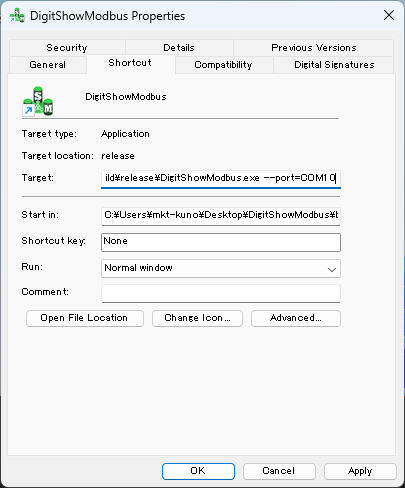
\includegraphics[width=0.9\hsize]{img/DSM_shortcut.png}
    \caption{ポート指定の例。\inlinecode{--port=COM10}や\inlinecode{-p=COM6}.}
\end{figure}

\section{実験前：アプリを開く}
ショートカットをクリックしてアプリを開きましょう。\cref{fig:dsm_main}のようなメイン画面が表示されます。値がすべて0の場合は、AD/DAボードとの通信がうまくできていないので、ポート指定を再確認してください。

\begin{figure}[htbp]
    \centering
    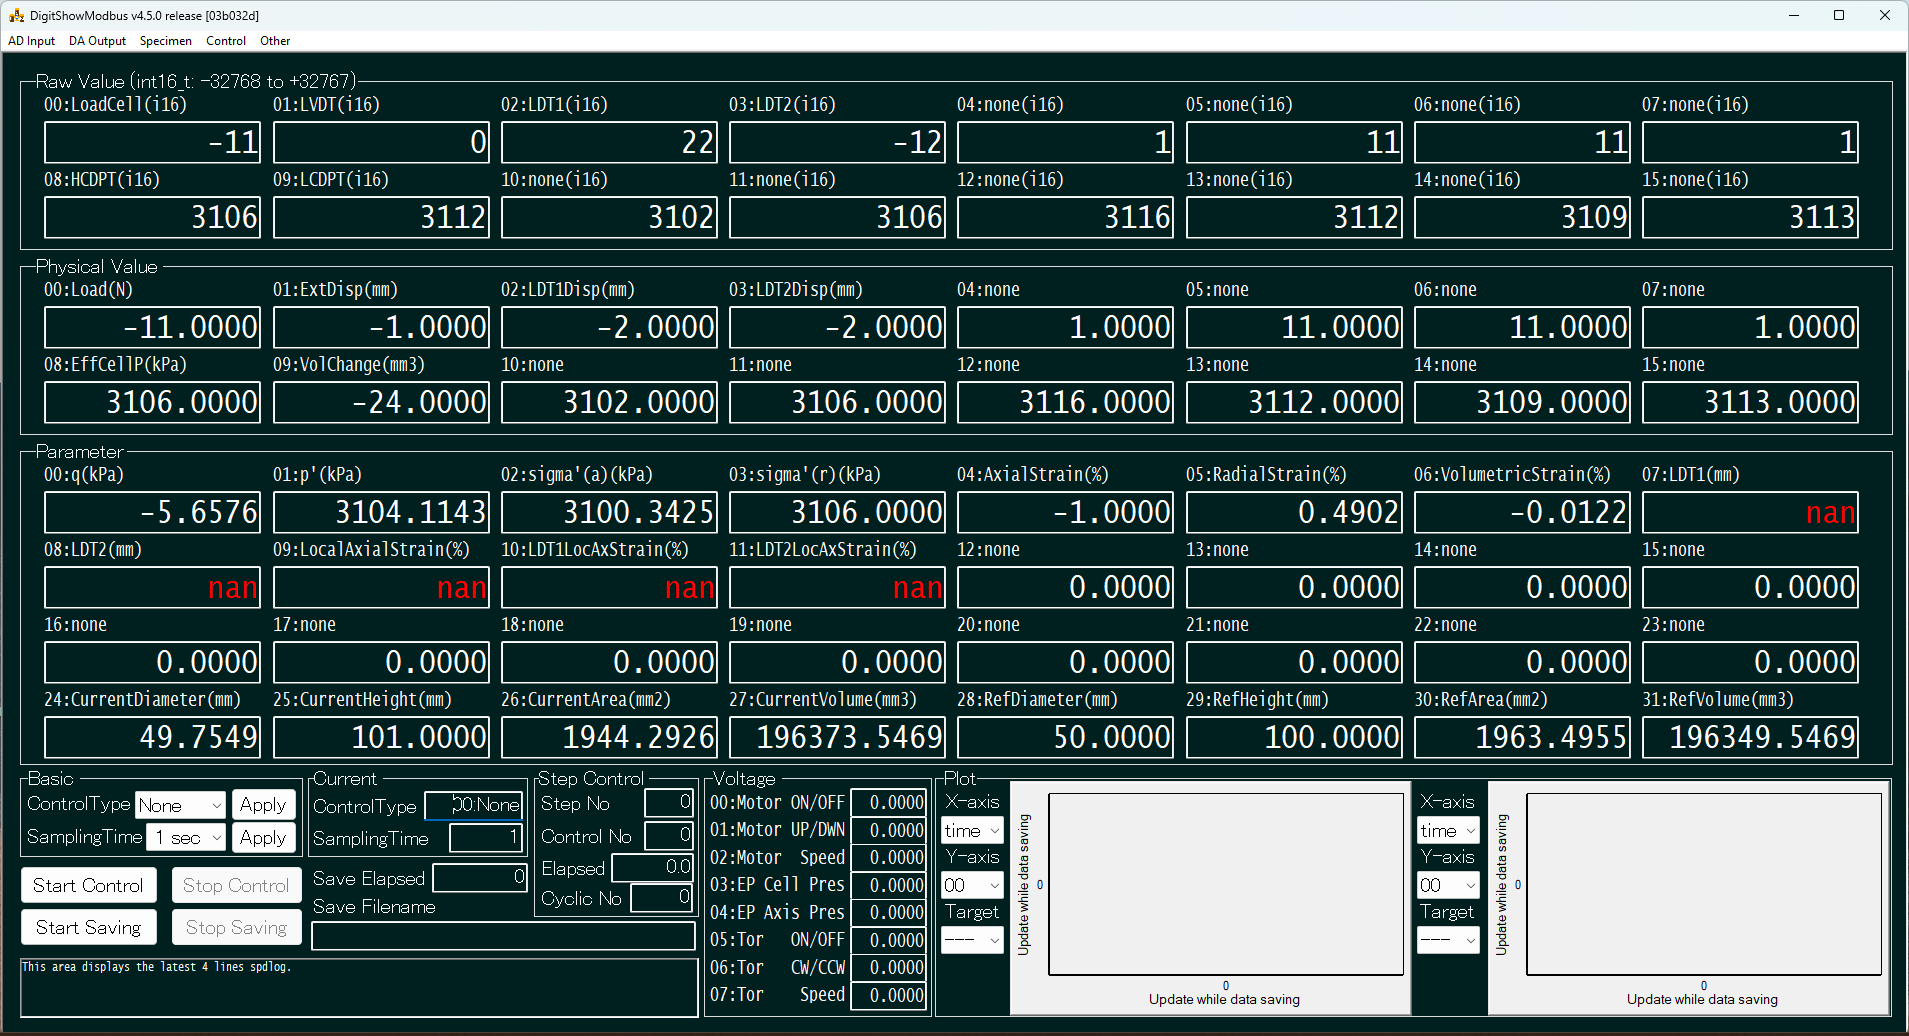
\includegraphics[width=0.9\hsize]{img/DSM_main.png}
    \caption{メイン画面。}
    \label{fig:dsm_main}
\end{figure}

\section{供試体を設置する前：ロードセルのキャリブレーション値の入力} \label{sec:loadcell_cal}
\begin{enumerate}
    \item 左上の``AD Input''タブで``Calibration Factors''をクリックします。
    \item キャリブレーション値を設定します。
    \begin{itemize}
        \item 手動で各チャンネルの値を入力する場合：a, b, cの係数に値を入力し、``Update Varients''を押します。
        \item ファイルを読み込む場合：``Load from a file''をクリックして、\inlinecode{.cal}ファイルを読み込みます。現在の設定を保存する場合、``Save to a file''で保存することができます。
    \end{itemize}
    \item カウンターバランスを取った状態で、ロードセルのゼロ点を調整をします。ロードセルのチャンネル（CH0）の``Zero''ボタンを押します。そのチャンネルのphysical valueが0になるように、自動的にキャリブレーション値の定数項（c）が変更されます。
\end{enumerate}
\begin{figure}[htbp]
    \centering
    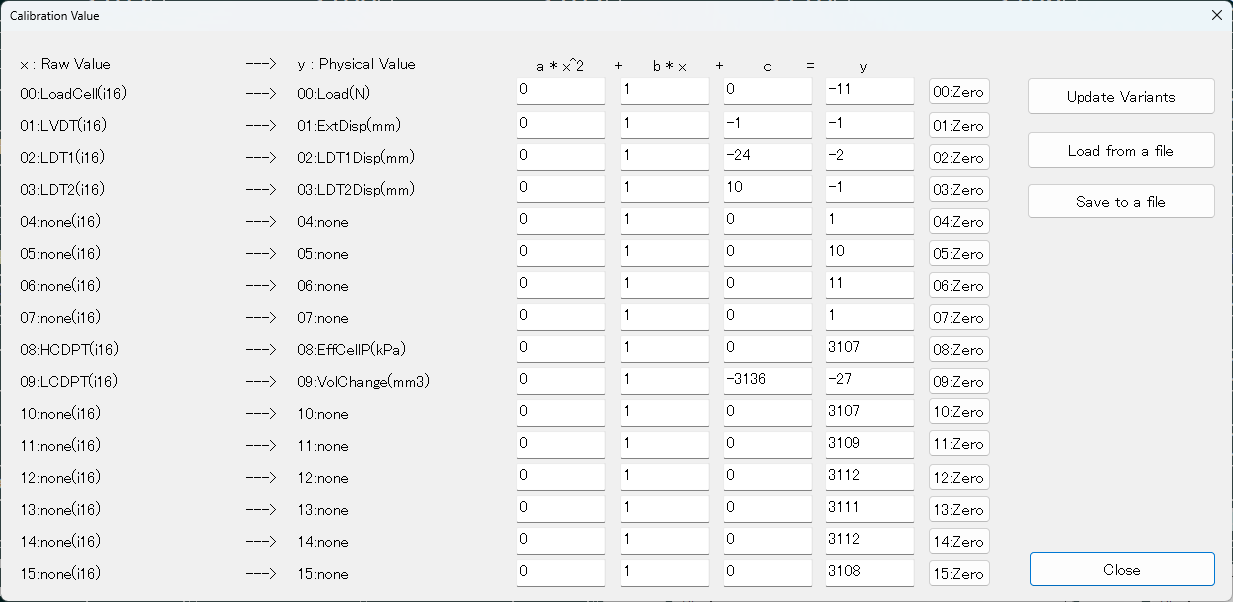
\includegraphics[width=0.9\hsize]{img/DSM_calib.png}
    \caption{各センサーのキャリブレーション値の入力画面。}
    \label{fig:dsm_calib}
\end{figure}

\section{供試体の寸法計測後：供試体初期寸法の入力}
\begin{enumerate}
    \item 左上の``Specimen''タブで``Config''をクリックします。
    \item ``Initial''列の``Diameter''行と``Height''行に、供試体の初期寸法と高さを入力し、``-> present''ボタンを押します。
\end{enumerate}
\begin{figure}[htbp]
    \centering
    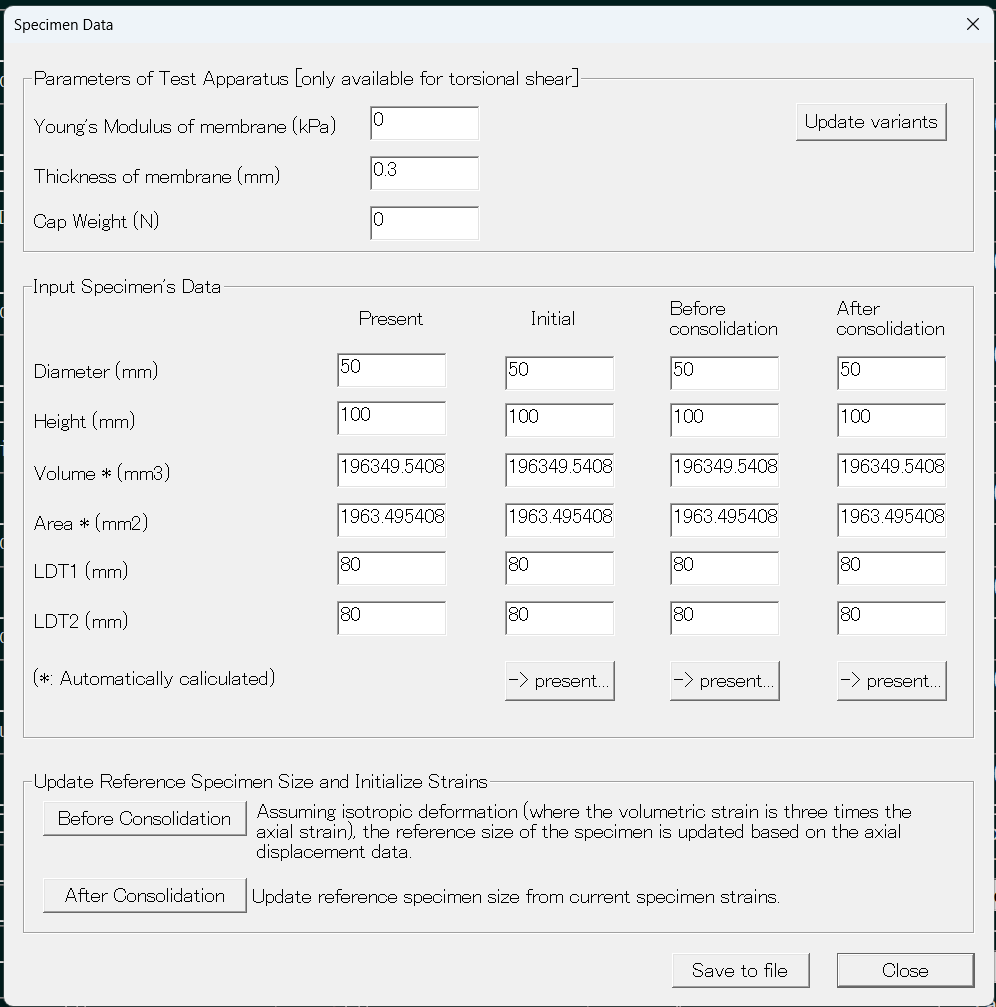
\includegraphics[width=0.9\hsize]{img/DSM_specimen.png}
    \caption{供試体の情報の入力画面。}
    \label{fig:dsm_specimen}
\end{figure}

\section{載荷装置と三軸セルを接続した後①：変位計のキャリブレーション値の入力}
\cref{sec:loadcell_cal}と同様にして、変位計（LVDT）のチャンネル（CH1）キャリブレーション値の入力およびゼロ点の調整を行います。

\section{載荷装置と三軸セルを接続した後②：Pre-Consolidation}
Pre-consolidationは所定の$q$（軸差応力$\ab[\unit{kPa}]$）を保つ制御コマンドです。主に供試体の飽和過程で使用します。デフォルトの設定では、$q=0$なので、等方状態になります。
\begin{enumerate}
    \item メイン画面左下の``Control ID''を 1 にして、``Set''をクリックします。
    \item メイン画面左下の``Start Control''を押すと、制御が始まります。軸受けのクランプを緩め忘れないように気を付けてください。
\end{enumerate}

\section{供試体の飽和後：差圧計のキャリブレーション値の入力}
\cref{sec:loadcell_cal}と同様にして、高容量差圧計（HCDPT、CH8）、低容量差圧計（LCDPT、CH9）のキャリブレーション値の入力およびゼロ点の調整を行います。

\section{圧密①：EPの出力調整}
圧密・載荷過程では、EP（電空レギュレータ）を用いてセル圧を自動で制御します。
\begin{enumerate}
    \item 左上の``D/A Output''タブで``Voltage Output''をクリックします。
    \item ``CH 3: EP Cell Pressure''に適当な値を入力して``Update''を押します。EPの出力を現在のセル圧に合わせてから、セルに接続します。
\end{enumerate}

\section{圧密②：ひずみの初期化（Before Consolidation）}
\begin{enumerate}
    \item 左上の``Specimen''タブで``Config''をクリックします。
    \item ``Before Consolidation''をクリックします。等方的な変形が生じた（軸ひずみの3倍の体積ひずみが生じた）と仮定して、変位計から得られる軸ひずみを基に、ひずみの初期化および変位計とLCDPTのゼロ点調整がなされます。
\end{enumerate}

\section{圧密③：Control from fileの設定}
\begin{enumerate}
    \item メイン画面左下の``Stop Control''を押して、制御を停止します。
    \item 左上の``Control''タブで``Control from file''をクリックします。
    \item 圧密・クリープ・軸圧縮の設定を入力します。``Load''を押すとその Step No. の現在の設定が表示され、``Update''を押すとそのStep No.の設定が現在入力している値（パラメータ）に更新されます。
    \item Current Step No. が圧密のstep（0）になっていることを確認してください。
    \item 設定の一例は\cref{tab:sample_table}の通りです（初期拘束圧\qty{20}{kPa}から、\qty{100}{kPa}で等方圧密し、排水条件で軸ひずみ\qty{15}{\percent}まで単調載荷する場合）：
    \begin{itemize}
        \item Step No.1 のCreepの時間は本来予定している時間よりも長くしておくことを推奨します（意図しないタイミングで次のstepに進むのを防ぐため）。
        \item 非排水軸圧縮（CU試験）を行う場合は、載荷中セル圧を変化させる必要がないため、Step No.2のMonotonic Axial LoadingのArgs[02]を0としてください。
        \item Motor RPMと軸変位速度の関係は事前にキャリブレーションしてください（試験機により異なります）。
        \item Control from fileという名前が示すように、タブで区切られた設定ファイルの読み込みや書き出しも可能です。
    \end{itemize}
    \begin{table}[htbp]
        \centering
        \caption{Control from file の設定例。}
        \begin{tabular}{rlrrrrrrr}
            \toprule
            Step No. & Control No. (name) & Para0 & Para1 & Para2 & Para3 & Para4 & Para5 & Para6 \\ \midrule
            0 & 5: Linear Stress Path Loading & 20 & 20 & 100 & 100 & 10 & 10 & 1000 \\
            1 & 4: Creep & 0 & 10 & 1000 & 10000 & 100 & - & - \\
            2 & 1: Monotonic Axial Loading & 0 & 300 & 100 & 1 & 15 & 0 & 0 \\ \bottomrule
        \end{tabular}
        \label{tab:sample_table}
    \end{table}
\end{enumerate}
\begin{figure}[htbp]
    \centering
    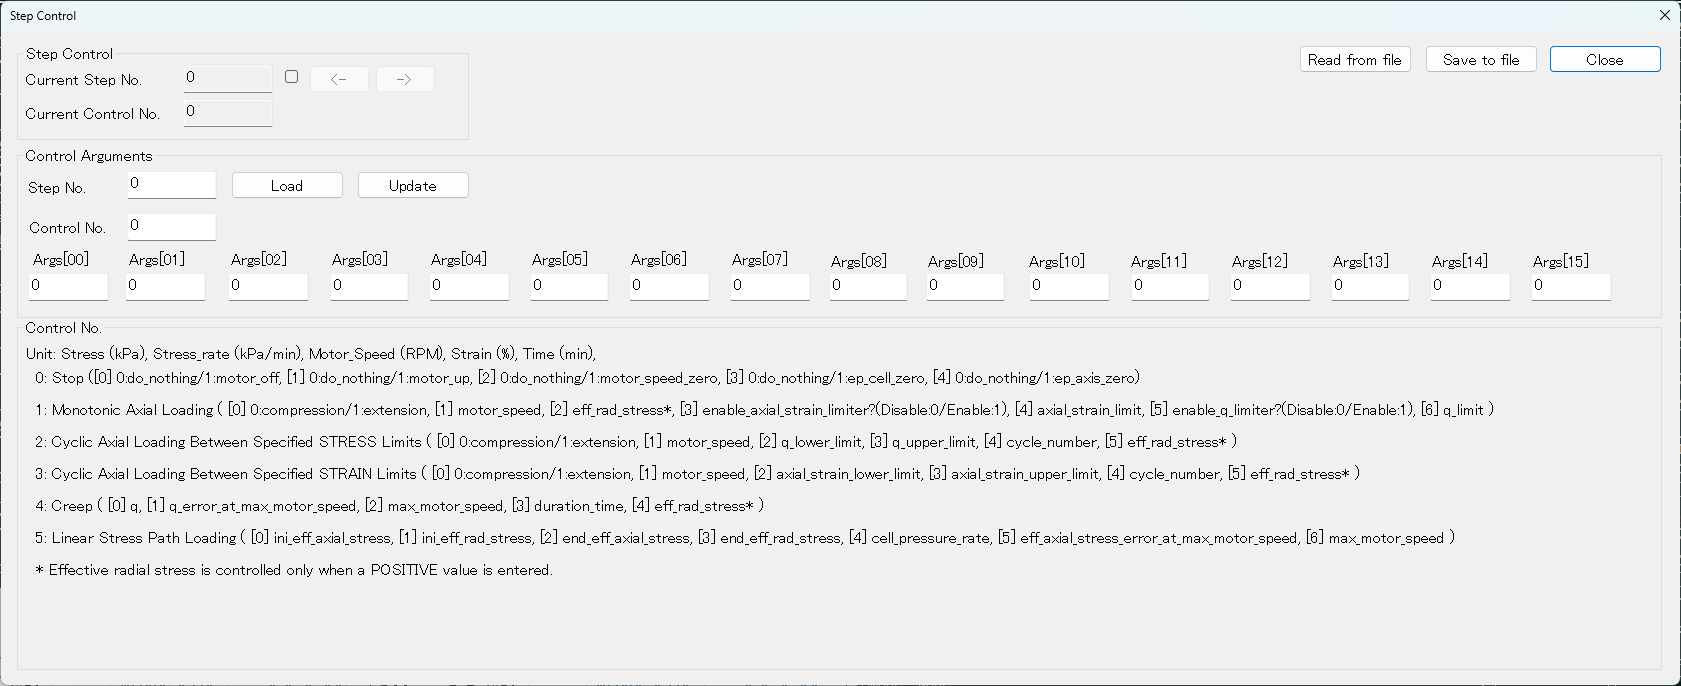
\includegraphics[width=0.9\hsize]{img/DSM_ctrl_file.png}
    \caption{制御の設定の入力画面。}
    \label{fig:dsm_ctrl_file}
\end{figure}


\section{圧密④：データ保存と制御の開始}
\begin{enumerate}
    \item メイン画面左下の``Control ID''を 15 にして``Set''をクリックします。
    \item メイン画面左下の``Start Saving''を押して、データの記録を開始します（ファイル名は半角英数字かつ特殊記号を使用しないことを推奨）。
    \item メイン画面左下の``Start Control''を押して、圧密を開始します。
\end{enumerate}

\section{軸圧縮①：データ保存、圧密の停止}
メイン画面で``Stop Saving''および``Stop Control''を押して、圧密中のデータの記録と制御を終了します。

\section{軸圧縮②：ひずみの初期化（After Consolidation）}
\begin{enumerate}
    \item 左上の``Specimen''タブで``Config''をクリックします。
    \item ``After Consolidation''をクリックします。現在の軸変位や体積変化をもとに、ひずみの初期化および変位計とLCDPTのゼロ点調整がなされます。
\end{enumerate}

\section{軸圧縮③：Step No の変更}
\begin{enumerate}
    \item 左上の``Control''タブで``Control from file''をクリックします。
    \item チェックボックスをクリックしてから、右矢印ボタンをクリックして、Step Noを2（軸圧縮の制御）に進めます。
\end{enumerate}

\section{軸圧縮④：データの保存、載荷の開始}
\begin{enumerate}
    \item ``Start Saving''を押して、データの記録を開始します（ファイル名は半角英数字かつ特殊記号を使用しないことを推奨）。
    \item ``Start Control''を押して、載荷を開始します（非排水条件で載荷する場合は、バルブを締めるのを忘れずに！）。
\end{enumerate}

\section{片付け}
\begin{enumerate}
    \item 軸圧縮が終わってStep Noが 3 に進んだら、メイン画面左下の``Stop Saving'', ``Stop Control''を押して、データの記録と制御を終了します。
    \item 左上の``Specimen''タブで``Config''をクリックし、``Save to file''ボタンを押して、供試体の情報をファイルに保存します。
    \item すべての片付けが終わったら、最後にアプリを閉じます。お疲れ様でした！
\end{enumerate}

\chapter{ユーザーマニュアル}
ここでは、クイックスタートで書かれなかった、特に試験を実施するうえで必要となりうる内容を含みます。

\section{動作モードと背景色}
ここでは、DigitShowModbusの動作モードと背景色について説明します。
DigitShowModbusは、以下の2つの動作モードを持ちます。
\begin{description}
    \item[生研式モータ動作モード] 生研式の三軸圧縮試験装置を用いて、飽和供試体の三軸圧縮試験を行うためのモードです。
    \item[生研式ねじり試験動作モード] 生研式の中空ねじりせん断試験装置を用いて、飽和供試体の中空ねじりせん断試験を行うためのモードです。まだ開発中です。
\end{description}
ねじり試験モードは未完成のため、現在は三軸圧縮試験モードのみが使用可能です。以下では、三軸圧縮試験モードについて説明します。

通常、DigitShowModbusの背景色は深緑色です。背景色が暗い赤色の場合、オリジナル版ではないことを示します。
本マニュアルはオリジナル版を対象としたものであり、オリジナル版以外の動作については、サポートできません。

\begin{figure}[H]
    \centering
    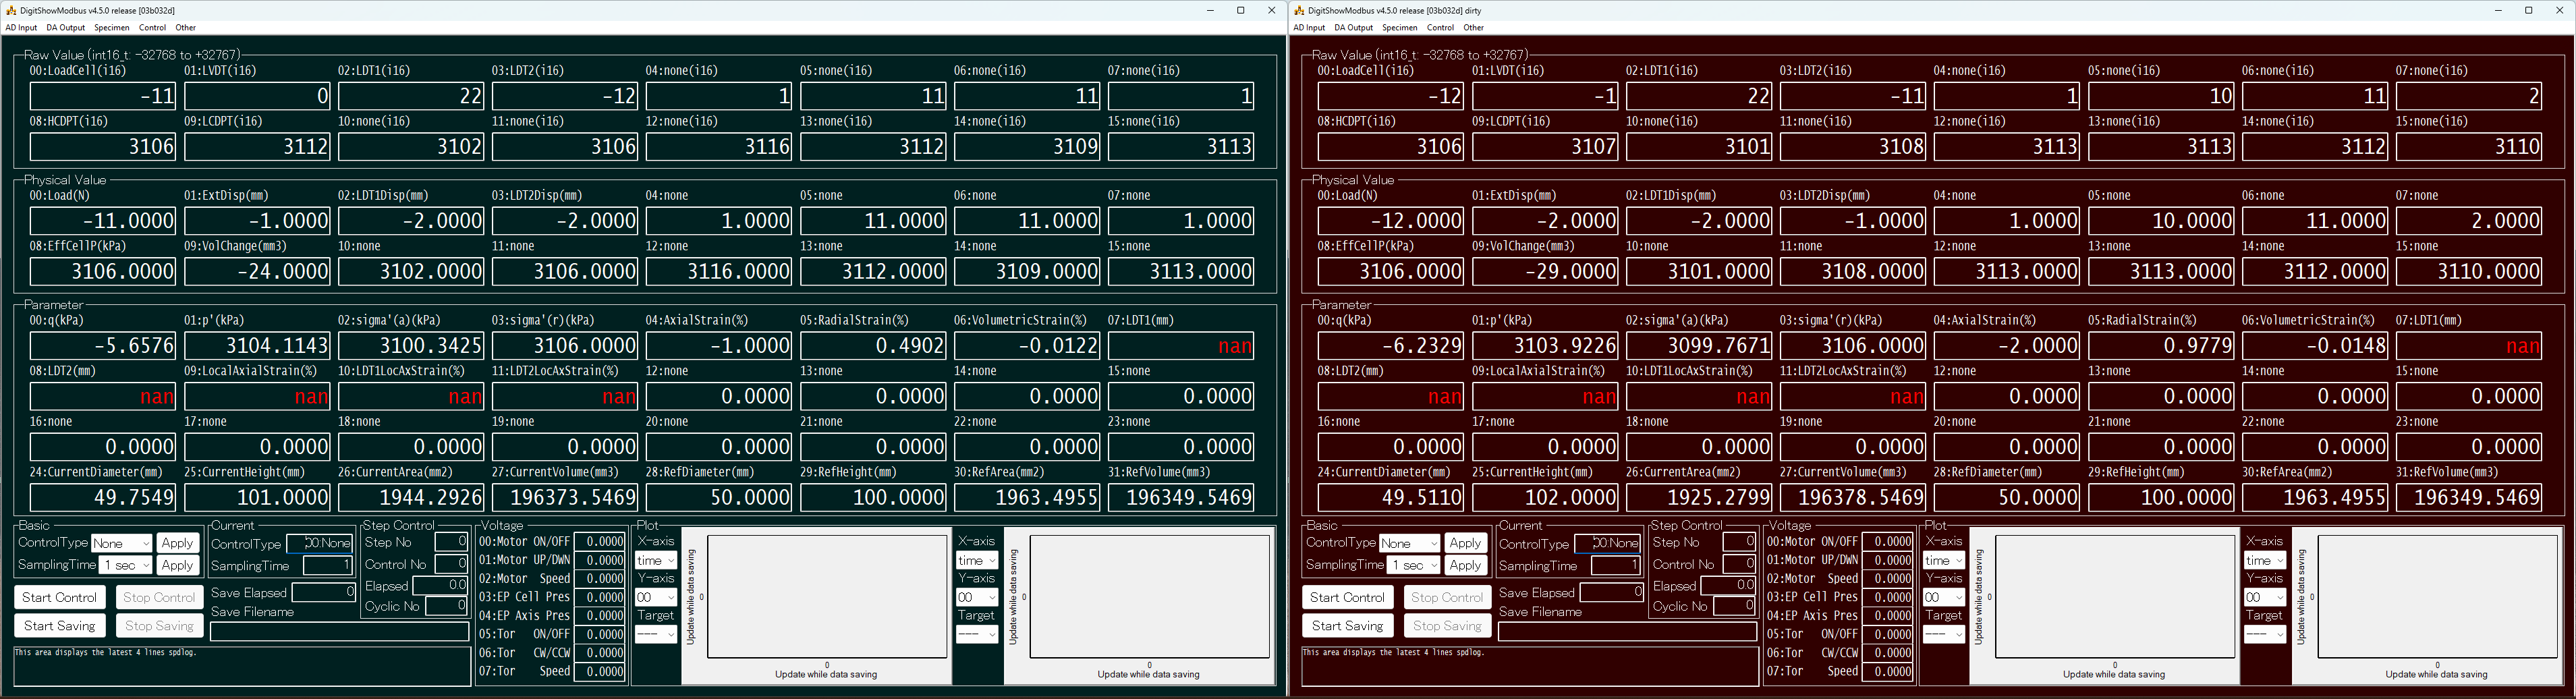
\includegraphics[width=0.9\hsize]{img/DSM_main_dirty.png}
    \caption{オリジナル版（左）と非オリジナル版（右）の背景色の違い}
\end{figure}

\section{起動時変数の設定（ユーザー向け）}
\label{sec:startup_variable_user}
ここでは、Windowsのショートカットのプロパティを利用した起動時変数の設定について、特に一般ユーザー向けのものに絞って説明します。
すべての起動時変数については、\cref{sec:startup_variable_developer}を参照してください。

起動時変数を設定するには、実行ファイル（DigitShowModbus.exe）のショートカットを作成し、ショートカットのプロパティを開いてください。
\emph{Target}で、実行ファイルのパスの後に、半角スペースを開けてから、以下に示す各種の起動時変数の指定を行ってください。

\begin{figure}[htbp]
    \centering
    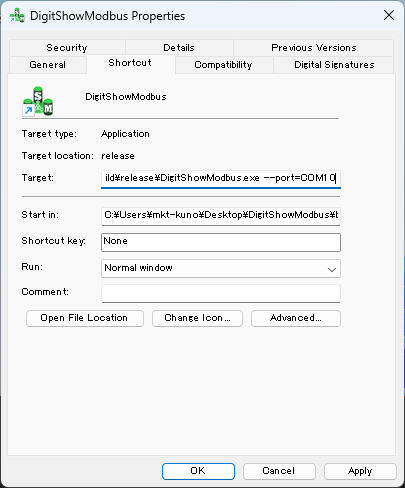
\includegraphics[width=0.9\hsize]{img/DSM_shortcut.png}
    \caption{ショートカットのプロパティを利用した起動時変数の設定例（ここでは\inlinecode{-p=COM3}でCOMポートを指定している）。}
\end{figure}

\subsection{ModbusRTU COM Port}
完全表記が\inlinecode{--port=}、短縮表記が\inlinecode{-p=}です。

ModbusRTUボードとの通信に使用するCOMポートを指定するための引数です。
\inlinecode{--port=COM10}や\inlinecode{-p=COM6}のように指定します。
ModbusRTUボードのうち、Trio（v1）・Quartet（v2）では、製造時期や互換ボードかどうかによって、FT232やCH340など、何かしらのUSBシリアル変換ICを使用しているため、デバイスマネージャー等で確認しましょう。
また、動作際してはドライバが必要になります。
ArduinoIDEをインストールするか、多くの場合WindowsUpdateのAdditional Updateでドライバがインストール可能です。
Yamanin（v3）では、USB-CDC（ACM）を使用した高速・高信頼のシリアル通信を採用しており、基本的にWindows標準のドライバが利用可能なため、追加のドライバインストールは不要です。
\begin{figure}[H]
    \centering
    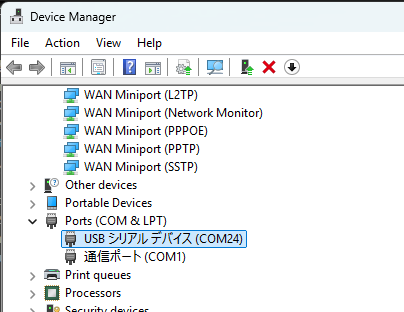
\includegraphics[width=0.6\hsize]{img/dev/device_manager.png}
    \caption{COMポートの例}
\end{figure}

\subsection{動作モード}
完全表記が\inlinecode{--mode=}、短縮表記が\inlinecode{-m=}です。

``0''もしくは``motor''を指定することで生研式モータ動作モードで起動します。

``1''もしくは``torsional''を指定することで生研式ねじり試験動作モードで起動します。

基本的にMotor動作モードで起動することをお勧めします。ねじりモードは開発中です。
Debugビルドで試用して、安全性を確認してから長期運用してください。

\subsection{クラッチ\&モータ動作電圧}
完全表記が\inlinecode{--invert\_motor\_enable=}、短縮表記が\inlinecode{-ime=}です。

完全表記が\inlinecode{--invert\_motor\_direction=}、短縮表記が\inlinecode{-imd=}です。

``True''もしくは``true''、``1''を指定することで極性が反転します。
デフォルト状態はソースコードの確認をしてください。大きな変更が加わっていない限りは、
``モータON''が``\SI{5.0}{[V]}''、``モータOFF''が``\SI{0.0}{[V]}''。
同じように``モータUP''が``\SI{5.0}{[V]}''、``モータDOWN''が``\SI{0.0}{[V]}''です。
コードを検索する場合は下記のような記述を探してください。
\begin{tcbcodeblock}{CDigitShowModbus.cpp より抜粋 }
    \begin{lstcodeblock}[language=C++]
#define AO_DEFAULT_VLT_MOTOR_ON		(5.0f)			// Voltage of Axial Motor ON
#define AO_DEFAULT_VLT_MOTOR_OFF	(0.0f)			// Voltage of Axial Motor OFF
#define AO_DEFAULT_VLT_MOTOR_UP		(5.0f)			// Voltage of Axial Motor UP
#define AO_DEFAULT_VLT_MOTOR_DOWN	(0.0f)			// Voltage of Axial Motor DOWN
\end{lstcodeblock}
\end{tcbcodeblock}

\subsection{Webサーバー機能}
完全表記が\inlinecode{--listen=}、短縮表記が\inlinecode{-l=}です。
地下実験室にいなくても、同一ネットワーク内であれば、研究室のパソコンからモニタリングが可能になります。
同一PCでたくさんチャートを見たいだけなら\inlinecode{--listen="localhost:80"}を、
実験室の他のパソコンからも見たいなら\inlinecode{--listen="0.0.0.0:80"}を設定してください。
\inlinecode{https://github.com/mkt-kuno/DigitShowWebview/}のRelease版をダウンロードして、
実行中の\inlinecode{DigitShowModbus.exe}と同じフォルダに置くと、簡単にリモートモニタリングが可能です。
複雑な表示がしたい人は自分でコーディングしてください。
フォルダ構成は以下のようになります。

\begin{tcbcodeblock}{Webサーバー機能有効時のフォルダ構成例}
    \begin{lstcodeblock}[]
DigitShowModbus.exe
modbus.dll
www/
├── index.html
├── ~~~~~.css
└── ~~~~~.js
    \end{lstcodeblock}
\end{tcbcodeblock}

\section{センサーと入力チャンネル構成}
ここでは標準的なセンサーと入力チャンネルの構成について説明します。
DigitShow Modbusでは、独自開発したModbusボードと通信を行い、センサーからアナログ信号を受け取ります。
CH0-7までがひずみゲージ式のセンサーの信号の受け取りに、CH8-15が0-5Vの直流電圧信号の受け取りに、それぞれ対応しています。
なお、センサーのキャリブレーション方法については、別のマニュアルを参照してください。

\subsection{CH0:ロードセル}
ロードセルは、供試体にかかる鉛直荷重を計測するためのセンサーです。4ゲージ（フルブリッジ）式で、セル室内のキャップ上部に取り付けられることが想定されます。

\subsection{CH1:LVDT（外部変位計）}
外部変位計は、供試体の鉛直変位を計測するためのセンサーです。4ゲージ（フルブリッジ）式で、セル室の外などに取付られることが想定されています。

\subsection{（任意）CH2,3:LDT（局所変位計）}
LDTはLocal Displacement Transducerの略で、Goto et al. (1991)によって開発された供試体の局所軸ひずみを計測するためのセンサーです。供試体側面上の2
点問の軸圧縮量から局所軸ひずみを求めます。ベディングエラー（「外部変位計などによってキャップや載荷ピストンの軸変位から求めた軸ひずみ」に含まれる測定誤差）の無い正確な軸ひずみを求めることができます。計測できる最大ひずみは1$\si{\percent}$程度ですが、微小なひずみを正確に計測することができます。供試体の直径方向に対称に1組設置し、2つのLDTで計測された値の平均値を用います。なお、LDTの設置は任意であり、使用しなくてもプログラムの動作に影響はありません。

\subsection{CH4-7:空きチャンネル}
ひずみゲージ式の各種センサーを接続することができる空きチャンネルです。

\subsection{CH8:HCDPT（高容量差圧計）}
供試体の半径方向の有効応力を計測するためのセンサーです。セル水の圧力と供試体の間隙水圧の差圧を測ります。差圧に応じた4-20mVのDC信号を伝送する差圧伝送器および、DC信号を直流電圧信号に変換するディストリビューターを使用することが想定されます。

\subsection{CH9:LCDPT（低容量差圧計）}
供試体の排水量を計測するためのセンサーです。排水量に応じて、供試体に繋がるビュレットの水位が変動するため、ビュレットの基準水位との水位差を差圧として計測します。HCDPTと同じく差圧伝送器とディストリビューターを使用することが想定されます。

\subsection{CH10-15:空きチャンネル}
直流電圧で入力される各種センサーを接続することができる空きチャンネルです。

\section{出力チャンネル構成}
\label{sec:output_channel}
DigitShow Modbusでは、独自開発したModbusボードと通信を行い、6チャンネルまたは8チャンネルの0-10Vのアナログ出力を使用することができます。
ここではアナログ出力チャンネルの構成について説明します。

\subsection{CH0:モーターON/OFF}
鉛直載荷モーターのクラッチのON/OFFを切り替えるための出力チャンネルです。デフォルトで、OFFのときは0V、ONのときは5Vが出力されます。\ref{sec:startup_variable_user}節に示す起動時変数の設定でON/OFF電圧の極性を反転させることができます。

\subsection{CH1:モーターUP/DOWN}
鉛直載荷モーターのUP/DOWNを切り替えるための出力チャンネルです。デフォルトで、UPのときは5V、DOWNのときは0Vが出力されます。\ref{sec:startup_variable_user}節に示す起動時変数の設定でUP/DOWNの極性を変更することができます。試験機により極性を反転させる必要があるので注意してください。

\subsection{CH2:モーター速度}
鉛直載荷モーターの回転速度（RPM）を設定するための出力チャンネルです。多くの生研式三軸試験機では、300RPM/Vとなっています。

\subsection{CH3:セルEP圧力}
EPは電空レギュレータ(Electrical-Pneumatic converter)の略称で、電圧に応じた空圧を出力する装置で、セル圧の制御に使用されます。デフォルトでは、0.01275kPa/Vの設定となっています。

\subsection{CH4-7:空きチャンネル}
生研式モータ動作モードでは、空きチャンネルとなります。

\section{供試体寸法・ひずみ・応力の計算式}
ここでは、DigitShow Modbusで計算される供試体寸法・ひずみ・応力の計算式について説明します。

\subsection{供試体寸法}
供試体寸法には、時々刻々と変化する現在の寸法のほかに、レファレンス値という概念が存在します。現在の寸法は、「どこからどのくらい増えた／減ったのか」を計算することによって得られますが、レファレンス値とは、この「どこから」の情報に相当します（「どのくらい増えた／減った」の情報はセンサーから得られます）。また、レファレンス値はひずみの計算の分母に用いられます。レファレンス値は時々刻々の変化はしない定数ですが、値は圧密の前と後で更新されます。

\subsubsection{供試体寸法のレファレンス値}
試験の最初に、実験者は供試体の初期直径を$d_\mathrm{init}$と初期高さ$h_\mathrm{init}$を測定します。これらをもとに初期体積$V_\mathrm{init}$が次のように計算されます。
\begin{align}
    V_\mathrm{init} = \frac{\pi{d_\mathrm{init}}^2h_\mathrm{init}}{4}
\end{align}

Before Consolidationを押す時点でのLVDTで計測された変位を$\delta_\mathrm{BC}$とします。等方的な変形が生じた（軸ひずみの3倍の体積ひずみが生じた）という仮定のもと、供試体寸法のレファレンス値（圧密前高さ$h_\mathrm{BC}$、圧密前体積$V_\mathrm{BC}$、圧密前直径$d_\mathrm{BC}$）は次のように更新されます。
\begin{align}
    h_\mathrm{BC} &= h_\mathrm{init} - \delta_\mathrm{BC} \\
    V_\mathrm{BC} &= V_\mathrm{init} \ab(1 - \frac{3\delta_\mathrm{BC}}{h_\mathrm{init}}) \\
    d_\mathrm{BC} &= \sqrt{\frac{4V_\mathrm{BC}}{\pi h_\mathrm{BC}}}
\end{align}

After Consolidationを押す時点でのLVDTで計測された変位を$\delta_\mathrm{AC}$と、LCDPTで計測された排水量を$W_\mathrm{AC}$とします。これらをもとに、圧密後の供試体寸法のレファレンス値（圧密前高さ$h_\mathrm{AC}$、圧密前体積$V_\mathrm{AC}$、圧密前直径$d_\mathrm{AC}$）は次のように更新されます。
\begin{align}
    h_\mathrm{AC} &= h_\mathrm{BC} - \delta_\mathrm{AC} \\
    V_\mathrm{AC} &= V_\mathrm{BC} - W_\mathrm{AC} \\
    d_\mathrm{AC} &= \sqrt{\frac{4V_\mathrm{AC}}{\pi h_\mathrm{AC}}}
\end{align}

\subsubsection{供試体の現在の寸法}
現在のレファレンスの高さを$h_\mathrm{ref}$、体積を$V_\mathrm{ref}$とします。また、LCDPTで計測された現在の排水量（供試体から出る方向が正）を$W$と、LVDTで計測された鉛直変位（供試体が圧縮する方向が正）を$\delta$とします。このとき、現在の供試体の高さ$h$, 体積$V$と断面積$A$は次のようになります。
\begin{align}
    h &= h_\mathrm{ref} - \delta \\
    V &= V_\mathrm{ref} - W \\
    A &= \frac{V}{h}
\end{align}

\subsection{ひずみ}
現在の高さを$h$、体積を$V$とし、レファレンス高さを$h_\mathrm{ref}$、体積を$V_\mathrm{ref}$とします。このとき、軸ひずみ$\varepsilon_\mathrm{a} \ \ab[\si{\percent}]$, 体積ひずみ$\varepsilon_\mathrm{v} \ \ab[\si{\percent}]$, 半径方向ひずみ$\varepsilon_\mathrm{r} \ \ab[\si{\percent}]$は次のように計算されます。
\begin{align}
    \varepsilon_\mathrm{a} &= \ab(1 - \frac{h}{h_\mathrm{ref}}) \times 100 \\
    \varepsilon_\mathrm{v} &= \ab(1 - \frac{V}{V_\mathrm{ref}}) \times 100 \\
    \varepsilon_\mathrm{r} &= \ab(1 - \sqrt{\frac{1-\varepsilon_\mathrm{v}}{1-\varepsilon_\mathrm{a}}}) \times 100
\end{align}

なお、昔のプログラム（DigitShowBasic）では、真ひずみが使用されていました。
地盤工学会の基準は公称ひずみを採用していたため、DigitShowModbusではよりシンプルに公称ひずみを採用しました。
ひずみ10\si{\percent}くらいまでであれば、両者の差は小さいですが、変形が大きくなるほど、公称ひずみ（現プログラム）と真ひずみ（旧プログラム）の差が大きくなります。既往研究との比較をする際には注意してください。
真ひずみはひずみの足し合わせができることが利点とされるようです。
必要に応じて、事後的に自分で計算してください。

\subsection{応力}
ロードセルが計測する荷重を$F$とします。軸差応力$q$は次式で計算されます。
\begin{align}
    q = \frac{F}{A}
\end{align}
HCDPTの計測する値がそのまま半径方向の有効応力${\sigma'}_\mathrm{r}$になります。これらを用いて、軸方向の有効応力${\sigma'}_\mathrm{a}$と平均有効応力$p'$は次のようになります。
\begin{align}
    {\sigma'}_\mathrm{a} &= {\sigma'}_\mathrm{r} + q \\
    p' &= \frac{{\sigma'}_\mathrm{a} + 2{\sigma'}_\mathrm{r}}{3} \\
    &= \frac{q + 3{\sigma'}_\mathrm{r}}{3}
\end{align}

\subsection{(LDTを使用した場合のみ)局所鉛直ひずみ}
LDT(Local Displacement Transducer)を使用した場合、鉛直方向の局所ひずみを計算することができます。LDTのレファレンス長さを$LDT_\mathrm{ref}$、LDTで計測された局所変位を$\delta_\mathrm{LDT}$とします。このとき、現在のLDTの長さ$LDT$と局所鉛直ひずみ$\varepsilon_\mathrm{LDT}$は次のように計算されます。
\begin{align}
    LDT &= LDT_\mathrm{ref} - \delta_\mathrm{LDT} \\
    \varepsilon_\mathrm{LDT} &= \ab(1 - \frac{LDT}{LDT_\mathrm{ref}}) \times 100
\end{align}
なお、LDTは、供試体のひねり状態の補正するために、供試体の直径方向に対象に1組設置し、2つのLDTで計測された$\varepsilon_\mathrm{LDT}$の平均値を用いることが推奨されます。

\section{各ウインドウの説明}
ソフトウェアの各ウインドウについて説明します。

\subsection{MainWindow}
起動時に表示されるメインウインドウの各部分の説明をします。
\begin{figure}[htbp]
    \centering
    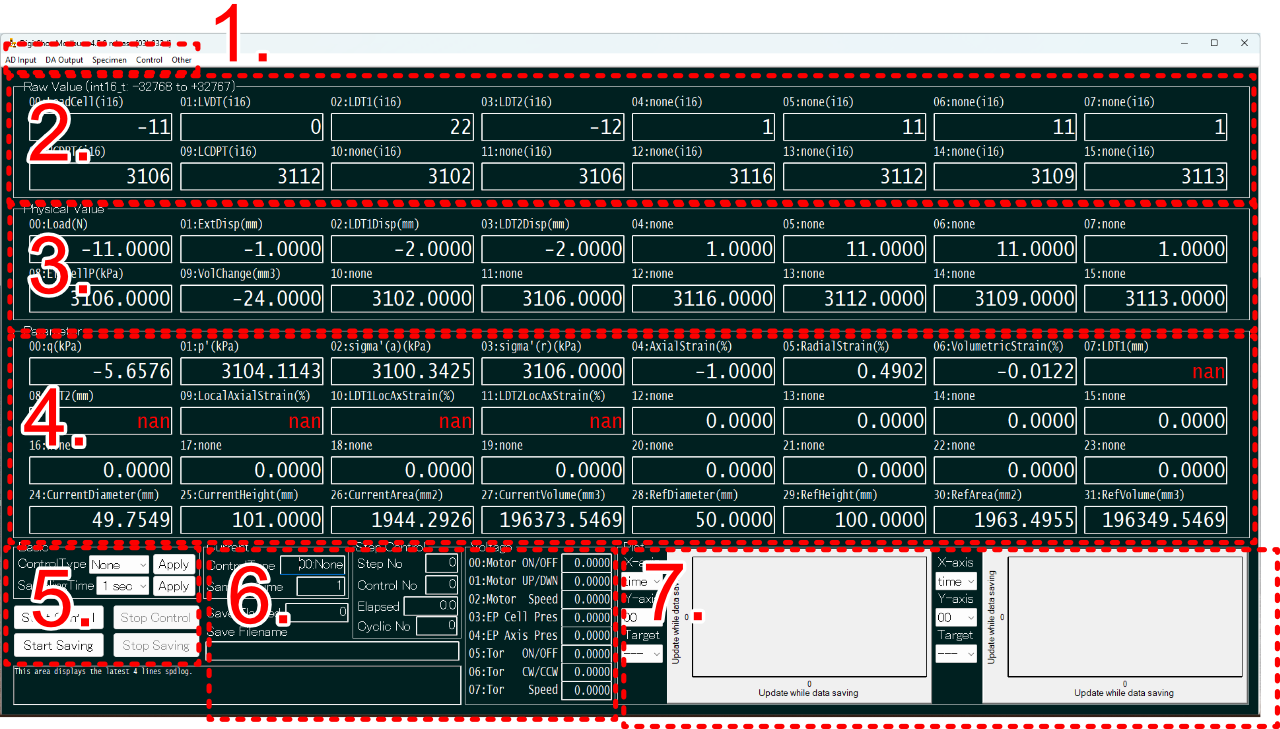
\includegraphics[width=0.9\hsize]{img/DSM_main_add_inst.png}
    \caption{メイン画面。}
    \label{fig:dsm_main_add_inst}
\end{figure}

\begin{enumerate}
    \item メイン画面の左上にあるタブから、キャリブレーションや供試体の情報、コントロール設定などに関する各ウィンドウ（次項以降で詳述）を開くことができます。
    \item Raw Valueでは、センサーからAD変換されたデジタル信号の生データを表示します。最小値は-32768、最大値は32767のint16型の値が表示されます。
    \item Physical Valueでは、Raw Valueをキャリブレーション値を用いて物理量($\si{N}$や$\si{mm}$など)に変換した値を表示します。
    \item Parametersでは、応力ひずみや、供試体の現在の寸法、レファレンス寸法などが表示されます。これらの値は、Physical Valueや供試体寸法の情報をもとに計算された値です。
    \item Basic Settingsでは、Control IDや、Samplingレートの設定や、制御とサンプリングの開始・停止を行うことができます。なお、Control IDやSamplingレートの設定は、Setボタンを押すことで反映されます。
    \item Current Settings \& Voltage Outputでは、現在の各種設定や\ref{sec:output_channel}節に示すアナログ電圧出力値の情報が表示されます。
    \item Plotでは、データ保存中のRaw ValueやPhysical Value、Parametersの値の変化をグラフで表示します。表示点数はデフォルト設定では最大512点までで、プロット間隔は自動的に調整されます。
\end{enumerate}

\subsection{DA Output - Voltage Output}
アナログ出力について、直接電圧を指定して出力できるウインドウです。
EPを三軸セルに接続する前に、EPの出力圧力を調整する際に使用します。
また、装置を組み上げたり接続し直した場合に、クラッチやモータなどの動作確認などにも使用されます。
\begin{figure}[htbp]
    \centering
    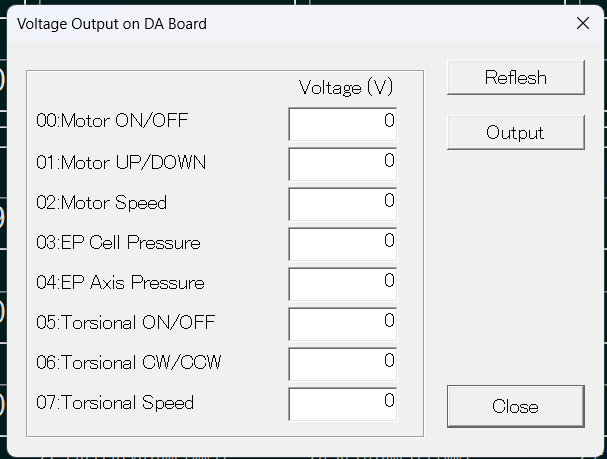
\includegraphics[width=0.6\hsize]{img/DSM_VoltOut.png}
    \caption{DA Output - Voltage Outputウィンドウ。}
    \label{fig:dsm_VoltOut}
\end{figure}

\subsection{Specimen - Config}
供試体の初期寸法を設定するウインドウです。供試体の直径と高さ・LDTの長さなどを入力します。
\begin{figure}[htbp]
    \centering
    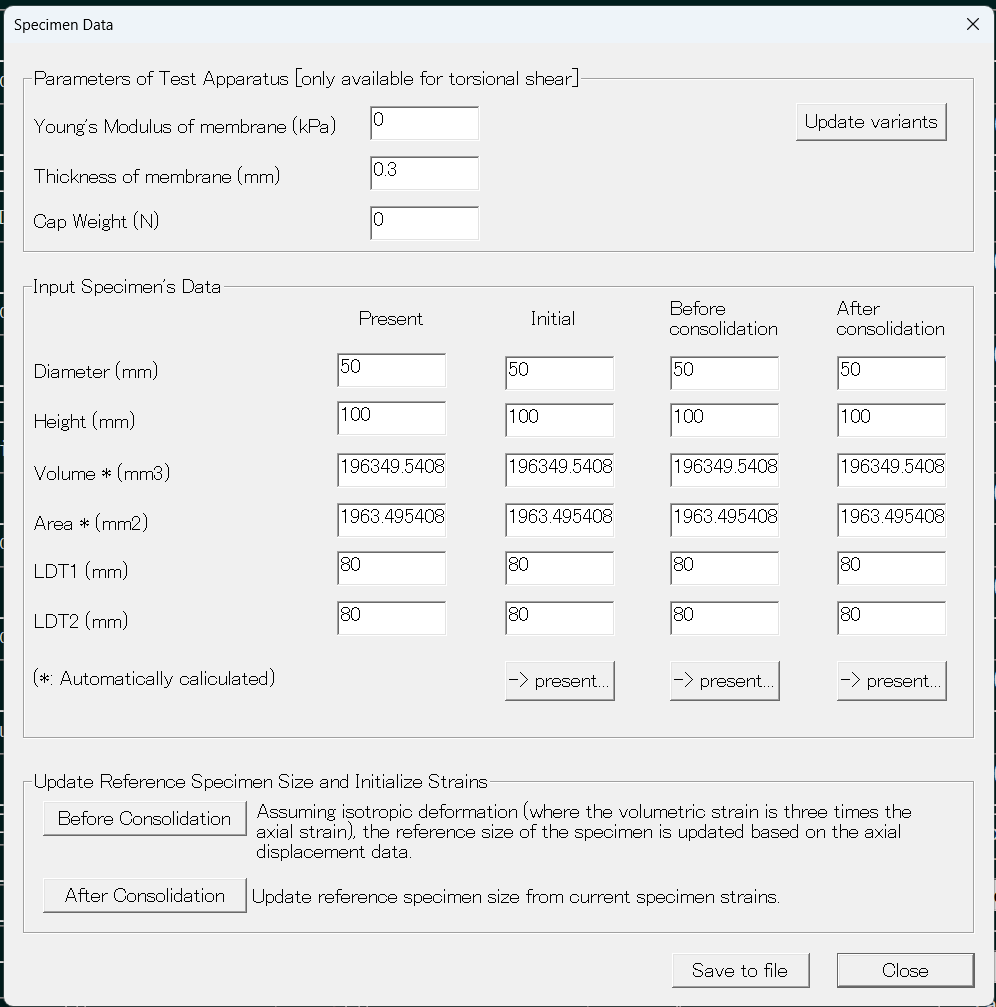
\includegraphics[width=0.7\hsize]{img/DSM_specimen.png}
    \caption{Specimen - Configウィンドウ。}
    \label{fig:dsm_SpecimenConfig}
\end{figure}
TDB...

\subsection{Control - Pre-Consolidation}
Pre-Consolidationは先行圧密用の制御コマンドです。主に供試体の飽和過程で使用します。
制御の詳細については、\cref{sec:control}を参照してください。
\begin{figure}[htbp]
    \centering
    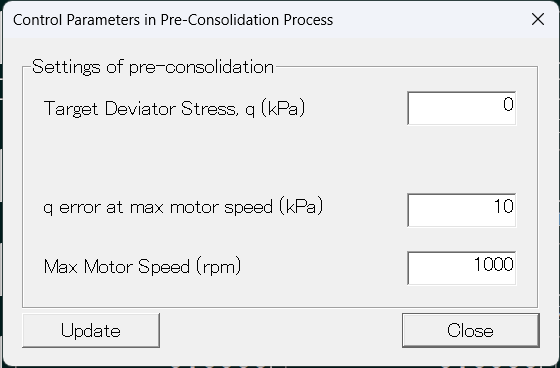
\includegraphics[width=0.4\hsize]{img/DSM_PreCons.png}
    \caption{Control - Pre-Consolidationウィンドウ。}
    \label{fig:dsm_PreCons}
\end{figure}

\subsection{Control - Control from file}
複数のコントロールを順序立てて自動的に行うための設定を行うウインドウです。圧密・クリープ・モーター速度・圧縮方向などの設定を入力します。
\begin{figure}[htbp]
    \centering
    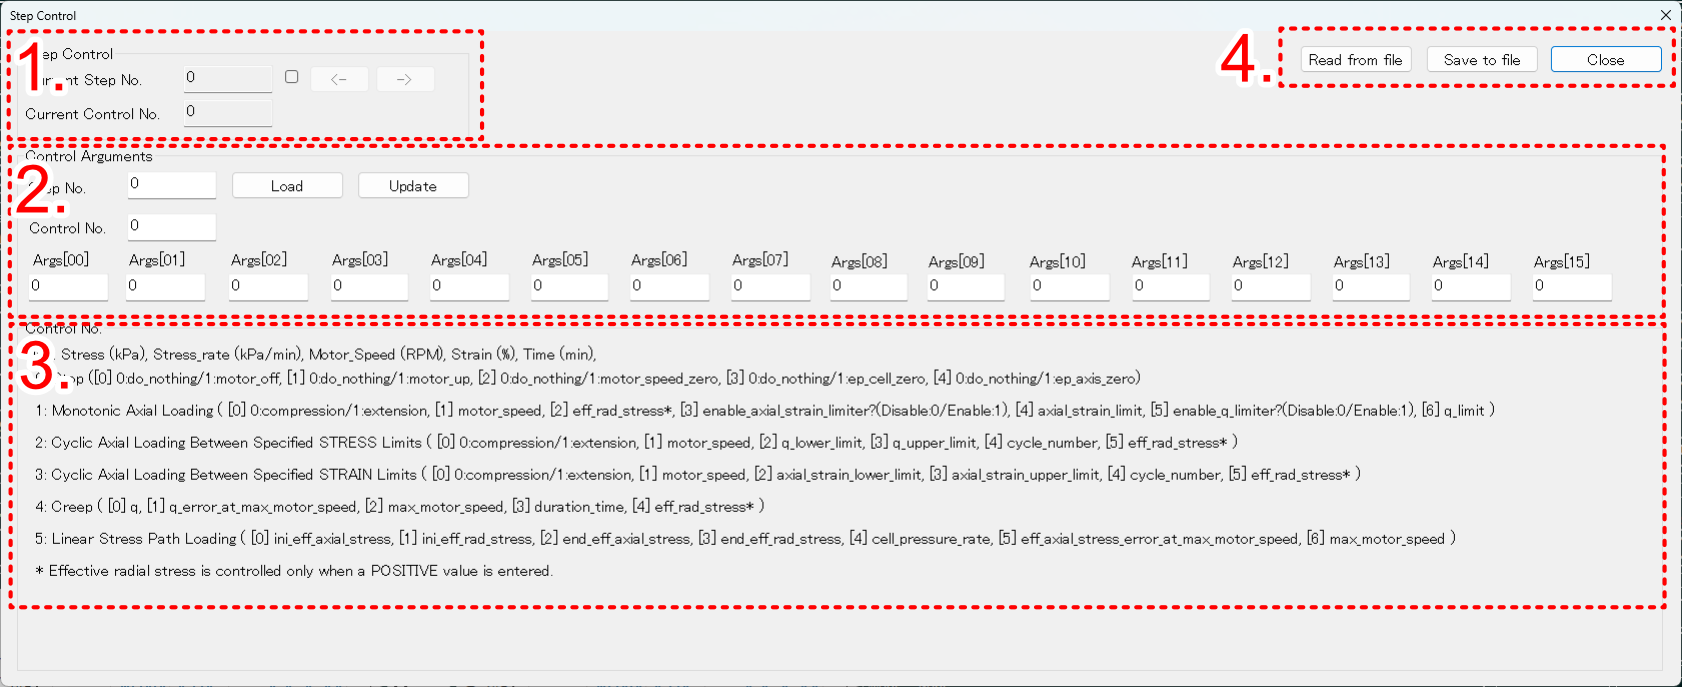
\includegraphics[width=0.9\hsize]{img/DSM_ctrl_file_add_inst.png}
    \caption{Control - Control from fileウィンドウ。}
    \label{fig:dsm_CtrlFile}
\end{figure}
\begin{enumerate}
    \item 現在のControlのStep No.が表示されます。チェックボックスを選択した上で、矢印ボタンをクリックするとStep No.のインクリメント・デクリメントができます。なお、設定可能なStep No.は0から1023までです。
    \item 各StepのControl No.の設定およびそのパラメータの設定を行うことができます。Loadボタンをクリックすると、現在入力中のStep No.の、DigitShowModbusに設定されているControl No.とパラメータが表示されます。Updateボタンをクリックすると、現在入力されているStep No.のControl No.とパラメータが、DigitShowModbus内に登録されます。
    \item 各Control No.の詳細が記述されています。なお、Control No.の詳細は、\cref{sec:control}を参照してください。
    \item Read from fileボタンをクリックすると、指定したファイルからStep No., Control No.とパラメータを読み込むことができます。Save to fileボタンをクリックすると、現在設定されているStep No., Control No.とパラメータの情報を、指定したファイルに保存することができます。Closeボタンを押すと、ウインドウが閉じます。
\end{enumerate}
制御の詳細については、\cref{sec:control}を参照してください。

\subsection{Other - Version}
ソフトウェアのバージョン情報を表示するウインドウです。
\begin{figure}[htbp]
    \centering
    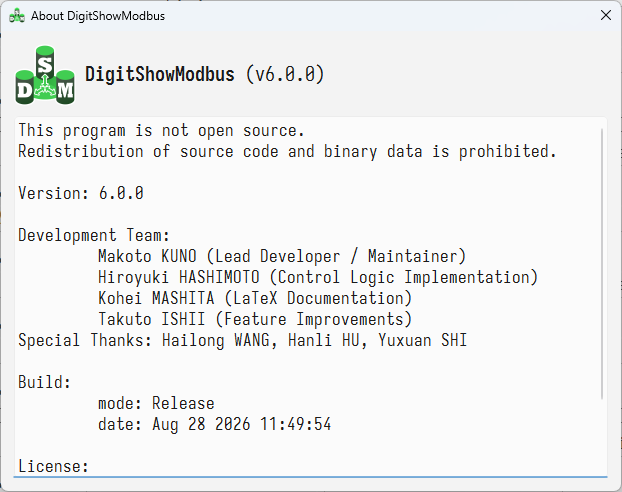
\includegraphics[width=0.6\hsize]{img/DSM_Version.png}
    \caption{Other - Versionウィンドウ。}
    \label{fig:dsm_Version}
\end{figure}

\subsection{Other - Environmental Variables}
ソフトウェアの環境変数を表示するウインドウです。
コントロール中やデータ保存中に、環境変数を確認したい場合は注意してください。
\begin{figure}[htbp]
    \centering
    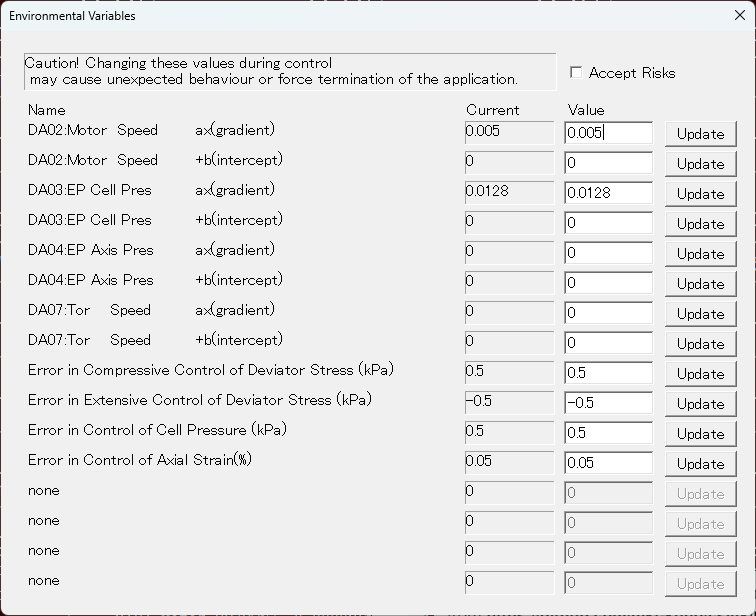
\includegraphics[width=0.6\hsize]{img/DSM_envval.png}
    \caption{Other - Environmental Variablesウィンドウ。}
    \label{fig:dsm_env}
\end{figure}

\subsection{Other - Open Log Folder}
ソフトウェアのログを表示するウインドウです。エラーが発生した場合などに参照します。

\subsection{Other - Open Config Folder}
ソフトウェアのが自動で生成する設定ファイルを表示するウインドウです。

\section{コントロールについて}
\label{sec:control}
ここでは、DigitShowModbusの各コントロール機能について説明します。
大きく分けて、供試体の飽和過程で使用するPre-Consolidation (Control ID:1)と、圧密や軸圧縮時に使用するControl from file (Control ID:15)の2つに分かれます。

\subsection{Pre-Consolidation}
Pre-Consolidationは、供試体の飽和過程で使用するコントロールです。
\cref{fig:precon-q-rpm}に示すように、設定した軸差応力を保つように載荷軸を上下させます。
デフォルトの設定では、$q=\qty{0}{\kPa}$なので、等方状態を保とうとします。

軸差応力が目標値から離れれば離れるほど、高速でモーターを回転させて載荷軸を上下させます（いわゆるP制御のようなもの）。
ただし、クラッチの消耗を防ぐため、軸差応力が\qty{0.5}{\kPa}以下しか離れていないのであれば、載荷軸は動かないようにプログラムされています（この閾値はユーザーからは設定できません）。
\begin{figure}
    \centering
    \begin{tikzpicture}
        % 原点の描画
        \draw[{Stealth[]}-] (0, 0) to[bend right] (-1.5, 1) node[left] {$\ab(\text{target\_deviator\_stress}, 0)$};
        % 座標軸の描画
        \draw[-{Stealth[]}] (-5, 0) -- (5, 0) node[below] {$q\ \ab[\unit{\kPa}]$};
        \draw[-{Stealth[]}] (0, -3) -- (0, 3) node[above right] {motor speed $\ab[\unit{RPM}]$};
        % q と motor speed の対応関係
        \draw[blue, ultra thick] (-5, -2.5) -- (-2.5, -2.5) -- (-1, -1);
        \draw[dashed] (-1, -1) -- (-1, 0);
        \draw[blue, ultra thick] (-1, 0) -- (1, 0);
        \draw[dashed] (1, 0) -- (1, 1);
        \draw[blue, ultra thick] (5, 2.5) -- (2.5, 2.5) -- (1, 1);
        % max motor speed
        \draw[dashed] (2.5, 2.5) -- (0, 2.5) node[below left] {max\_motor\_speed};
        \fill (0, 2.5) circle (0.75mm);
        % モーターを動かさない閾値
        \draw[dashed] (2.5, 2.5) -- (2.5, 0);
        \draw[{Stealth[]}-{Stealth[]}] (0, -0.4) -- (1, -0.4) node[midway, below] {0.5};
        % q error at max motor speed
        \draw[{Stealth[]}-{Stealth[]}] (0, 0.4) -- (2.5, 0.4) node[right] {q\_error\_at\_max\_motor\_speed};
    \end{tikzpicture}
    \caption{Pre-Consolidationの動作のイメージ}
    \label{fig:precon-q-rpm}
\end{figure}

\subsection{Control from file - 0: No Control}
Control No.0: No controlは、何の制御も行いません。デフォルトの制御として設定されています。
モーターのクラッチはONのまま、モーターは回転しません（載荷軸は全く動きません）。
セル圧を制御するEPの出力電圧は、それまでの値を保持します（セル圧も基本的に変動しません）。

\subsection{Control from file - 1: Monotonic Axial Loading}
Control No.1: Monotonic Axial Loadingは、単調軸圧縮・軸伸長を行うコントロールです。

以下のパラメータが設定できます。
\begin{itemize}
    \item Args[00]: 圧縮(compression)か伸長(extension)か。0が圧縮、1が伸長です。
    \item Args[01]: モーターの回転速度。単位はRPM。RPMと実際の載荷速度の関係は試験機および減速機の設定などによって異なるため、予め確認しておく必要があります。
    \item Args[02]: 半径方向の有効応力。単位はkPa。正の値が入力されたときのみ、EPでセル圧を制御することで、円周方向の有効応力を設定された値に保ちます（0以下の値が入力された場合、EPの出力圧力は変化しません）。逆に、非排水三軸試験を行う場合には、必ず0を入力してください。
    \item Args[03]: 軸ひずみのリミッター設定を行うか否か。1で有効化、0で無効化。リミッターを有効化した場合、Args[04]で設定された値を超えるひずみが計測された場合に次のStep No.に進みます。
    \item Args[04]: 軸ひずみのリミッター値。単位は\si{\percent}。Args[03]でリミッターを有効化した場合に、Args[04]で設定された値を超えるひずみが計測された場合に次のStep No.に進みます。
    \item Args[05]: 軸差応力のリミッター設定を行うか否か。1で有効化、0で無効化。リミッターを有効化した場合、Args[06]で設定された値を超える軸差応力が計測された場合に次のStep No.に進みます。
    \item Args[06]: 軸差応力のリミッター値。単位はkPa。Args[05]でリミッターを有効化した場合に、Args[06]で設定された値を超える軸差応力が計測された場合に次のStep No.に進みます。
\end{itemize}
なお、Args[03]とArgs[05]のリミッターは少なくとも1つは設定する必要があります。両方とも設定しない場合、載荷が行われません。
また、非排水三軸圧縮試験の場合には、Args[04]にロードセルの定格容量を設定することをお勧めします（応力経路で限界状態線上に達したのちに軸差応力が増加し続ける場合があるためです）。

\subsection{Control from file - 2: Cyclic Axial Loading Between Specified STRESS Limits}
Control No.2: Cyclic Axial Loading Between Specified STRESS Limitsは、指定した応力範囲での繰り返し軸載荷を行うコントロールです。

以下のパラメータが設定できます。
\begin{itemize}
    \item Args[00]: 圧縮(compression)か伸長(extension)か。0が圧縮、1が伸長です。
    \item Args[01]: モーターの回転速度。単位はRPM。RPMと実際の載荷速度の関係は試験機および減速機の設定などによって異なるため、予め確認しておく必要があります。
    \item Args[02]: 軸差応力の下限値。単位はkPa。
    \item Args[03]: 軸差応力の上限値。単位はkPa。
    \item Args[04]: 何サイクル載荷を行うか。所定のサイクル数の載荷を終えた場合、次のStep No.に進みます。
    \item Args[05]: 半径方向の有効応力。単位はkPa。正の値が入力されたときのみ、EPでセル圧を制御することで、円周方向の有効応力を設定された値に保ちます（0以下の値が入力された場合、EPの出力圧力は変化しません）。逆に、非排水三軸試験を行う場合には、必ず0を入力してください。
\end{itemize}

\subsection{Control from file - 3: Cyclic Axial Loading Between Specified STRAIN Limits}
Control No.3: Cyclic Axial Loading Between Specified STRAIN Limitsは、指定した軸ひずみの範囲での繰り返し軸載荷を行うコントロールです。以下のパラメータが設定できます。
\begin{itemize}
    \item Args[00]: 圧縮(compression)か伸長(extension)か。0が圧縮、1が伸長です。
    \item Args[01]: モーターの回転速度。単位はRPM。RPMと実際の載荷速度の関係は試験機および減速機の設定などによって異なるため、予め確認しておく必要があります。
    \item Args[02]: 軸ひずみの下限値。単位は\si{\percent}。
    \item Args[03]: 軸ひずみの上限値。単位は\si{\percent}。
    \item Args[04]: 何サイクル載荷を行うか。所定のサイクル数の載荷を終えた場合、次のStep No.に進みます。
    \item Args[05]: 半径方向の有効応力。単位はkPa。正の値が入力されたときのみ、EPでセル圧を制御することで、円周方向の有効応力を設定された値に保ちます（0以下の値が入力された場合、EPの出力圧力は変化しません）。逆に、非排水三軸試験を行う場合には、必ず0を入力してください。
\end{itemize}

\subsection{Control from file - 4: Creep}
Control No.4: Creepは、クリープを行うコントロールです。
主に、Control No.5: Linear Stress Path Loadingを用いて圧密した後に、二次圧密を完了させるために使用されます。

以下のパラメータが設定できます。

\begin{itemize}
    \item Args[00]: ターゲットとなる軸差応力。単位はkPa。
    \item Args[01]: 軸差応力が現在の値とどれだけズレたときに、Args[02]で設定したモーターの回転速度となるか。単位はkPa。
    \item Args[02]: モーターの最大回転速度。単位はRPM。
    \item Args[03]: 継続時間。単位は分。指定した時間が経過した場合、次のStep No.に進みます。
    \item Args[04]: 半径方向の有効応力。単位はkPa。正の値が入力されたときのみ、EPでセル圧を制御することで、円周方向の有効応力を設定された値に保ちます（0以下の値が入力された場合、EPの出力圧力は変化しません）。逆に、非排水条件の場合には、0を入力してください。
\end{itemize}
実際の運用では、Args[03]には、十分長い時間を設定しておくことが多いです。これは、圧密→クリープ（二次圧密）の後、軸圧縮に進む前に、供試体のレファレンス値の更新とひずみの初期化の操作を手動で行う必要があるため、勝手に次のStep No.に進まないようにするためです。

また、Args[01]とArgs[02]は比例制御に関連するパラメータです。
軸差応力のエラー値（目標値と現在の値の差）とモーターの回転方向・速度の関係については、Pre-Consolidationを参照してください。

\subsection{Control from file - 5: Linear Stress Path Loading}
Control No.5: Linear Stress Path Loadingは、指定した応力経路に沿った載荷を行う始点となる応力状態と、終点となる応力状態を指定することで、応力経路上でその2点を結ぶ直線に沿った載荷を行うコントロールです。
一般に圧密時に使用されます。

以下のパラメータが設定できます。
\begin{itemize}
    \item Args[00]: 初期の軸（鉛直）方向の有効応力。単位はkPa。
    \item Args[01]: 初期の半径（水平）方向の有効応力。単位はkPa。
    \item Args[02]: 最終的に目標とする軸（鉛直）方向の有効応力。単位はkPa。
    \item Args[03]: 最終的に目標とする半径（水平）方向の有効応力。単位はkPa。
    \item Args[04]: セル圧を変化させる速度。単位はkPa/min。Args[01]からArgs[03]に向かって、指定した速度でセル圧が増加または減少します。
    \item Args[05]: 軸方向の有効応力が現在の目標値とどれだけズレたときに、Args[06]で設定したモーターの回転速度となるか。単位はkPa。
    \item Args[06]: モーターの最大回転速度。単位はRPM。
\end{itemize}
なお、Args[05]とArgs[06]は比例制御に関連するパラメータです。
有効応力のエラー値（現在の目標値と現在の実際の値の差）とモーターの回転方向・速度の関係については、Pre-Consolidationを参照してください。
\chapter{デベロッパーマニュアル}
この章ではハードウェア設計者、ソフトウェア開発者向けの情報を記載します。
DigitShowModbusのビルド方法や、専用のModbusRTUボードについて、装置開発に必要な情報が含まれています。

\section{起動時変数}
\label{sec:startup_variable_developer}
\subsection{ModbusRTU AD/DA Board}

2つの起動引数が存在します。
通信方法が``USBシリアル変換IC''か、``USB CDC-ACMによるマイコンとのダイレクト通信''かの選択が１つめ。
AnalogInputのInputRegisterが ``int16\_t'' か、``float32\_t'' かの選択が２つめです。

USB CDC-ACMによるダイレクト通信での高速ポーリング処理の有効化には
完全表記が\inlinecode{--usb\_cdc\_direct=}、短縮表記が\inlinecode{-ucd=}です。
``True''もしくは``true''、``1''を指定することで高速ポーリングが有効になります。

InputRegisterの精度をfloat32\_t（FloatInputRegister）にすると、
int16\_t で通信されるデータに、小数点以下の値を拡張する形で通信されます。
その為、キャリブレーションなどに影響はありません。
完全表記が\inlinecode{--float\_intput\_reg=}、短縮表記が\inlinecode{-fir=}です。
``True''もしくは``true''、``1''を指定することでInputRegisterの精度がfloat32\_tになります。

大まかな動作の違いを以下に示します。
\begin{table}[htbp]
    \centering
    \caption{各ボードの機能概要}
    \begin{tabular}{rlrrrr}
        \toprule
        BoardName & AD & DA & CDC-Direct & FloatInput & Other \\ \midrule
        Trio（v1） & 16 & 6 & False & False  & \\
        Quartet（v2） & 16 & 8 & False & False & \\
        Yamanin（v3） & 16 & 8 & True & True & \\
        Milia (v4) & 16 & 8 & True & True & \\
        Modulo (v5) & 16 & 8 & True & False & \\ \bottomrule
    \end{tabular}
    \label{tab:board_version}
\end{table}

\begin{figure}[H]
    \centering
    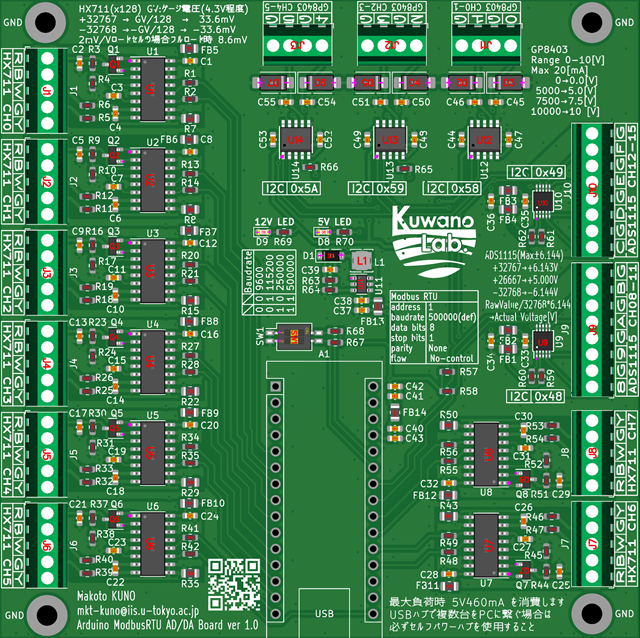
\includegraphics[width=0.5\hsize]{img/dev/trio.png}
    \caption{Trio（v1）ボード}
\end{figure}
ボードは緑で、上部DA出力コネクタが3個（6ch）なのが特徴です。

\begin{figure}[H]
    \centering
    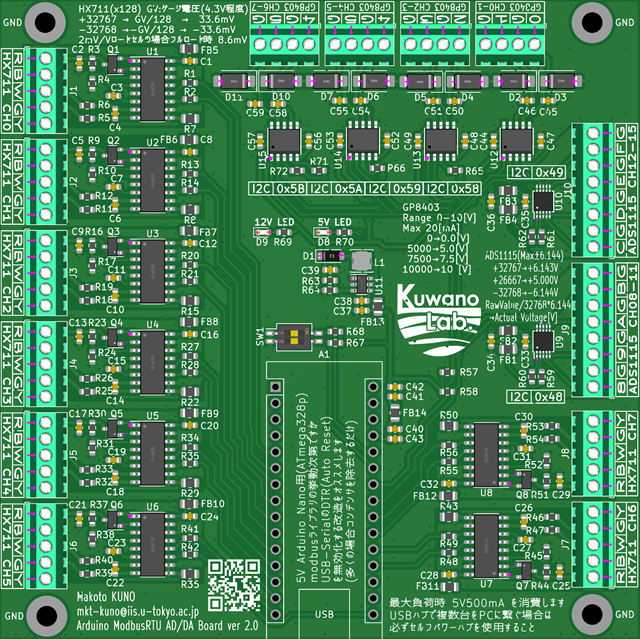
\includegraphics[width=0.5\hsize]{img/dev/quartet.png}
    \caption{Quartet（v2）ボード}
\end{figure}
ボードは緑で、上部DA出力コネクタが4個（8ch）なのが特徴です。

\begin{figure}[H]
    \centering
    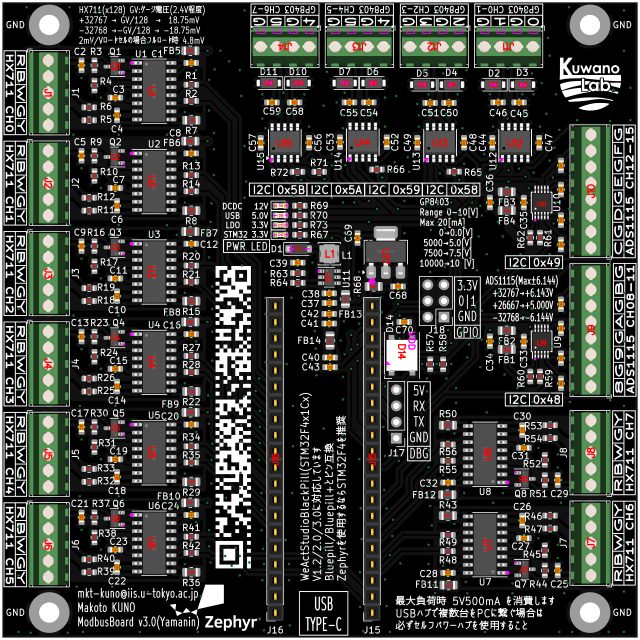
\includegraphics[width=0.5\hsize]{img/dev/yamanin.png}
    \caption{Yamanin（v3）ボード}
\end{figure}
ボードが黒く、Zephyrのロゴが入っており、NeoPixel LEDが搭載されていること、DA出力の付近の素子が小型化されていることが特徴です。

\begin{figure}[H]
    \centering
    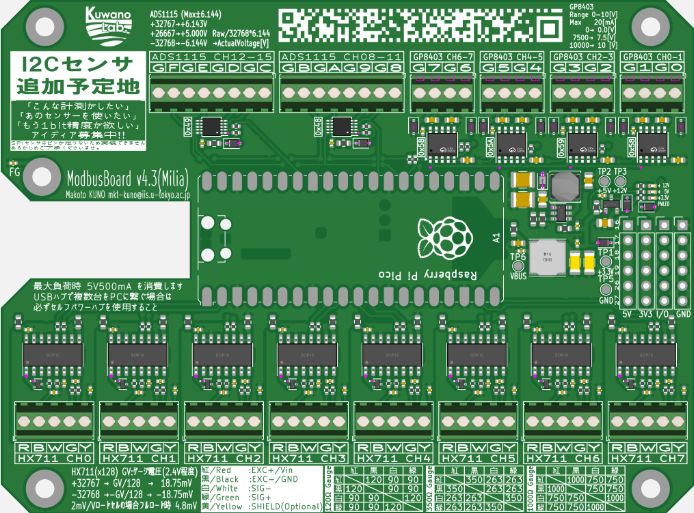
\includegraphics[width=0.5\hsize]{img/dev/milia.png}
    \caption{Milia（v4）ボード}
\end{figure}
ボードが正方形でなくなり、下側にHX711、上側にその他I/Oがまとめられていることが特徴です。

\subsection{ModbusRTU COM Port}
完全表記が\inlinecode{--port=}、短縮表記が\inlinecode{-p=}です。

ModbusRTUボードとの通信に使用するCOMポートを指定するための引数です。
\inlinecode{--port=COM10}や\inlinecode{-p=COM6}のように指定します。
Trio（v1）・Quartet（v2）では、製造時期や互換ボードかどうかによって、FT232やCH340など、何かしらのUSBシリアル変換ICを使用しているため、デバイスマネージャー等で確認しましょう。
また、動作際してはドライバが必要になります。
ArduinoIDEをインストールするか、多くの場合WindowsUpdateのAdditional Updateでドライバがインストール可能です。
Yamanin（v3）では、USB-CDC（ACM）を使用した高速・高信頼のシリアル通信を採用しており、基本的にWindows標準のドライバが利用可能なため、追加のドライバインストールは不要です。
\begin{figure}[H]
    \centering
    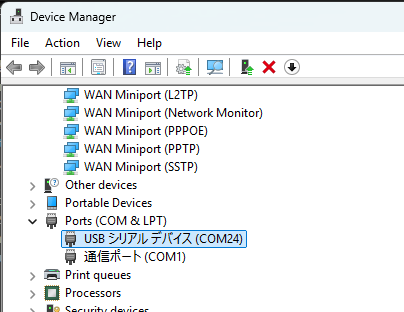
\includegraphics[width=0.6\hsize]{img/dev/device_manager.png}
    \caption{COMポートの例}
\end{figure}

\subsection{ModbusRTU Baudrate}
完全表記が\inlinecode{--baudrate=}、短縮表記が\inlinecode{-b=}です。
ModbusRTUボードとの通信速度を指定するための引数です。基本的に設定する必要はありません。
Trio・Quartet・YamaninではないオリジナルのModbusボードを使用する際に利用してください。

\subsection{フォント}
完全表記が\inlinecode{--font=}、短縮表記が\inlinecode{-f=}です。
フォントの指定は、\inlinecode{--font="MS Gothic"} \inlinecode{--font="Source Han Code JP"}のように指定します。
デフォルトは``Lucida Sans Typewriter''ですが、他のフォントを指定することも可能です。
見やすさもありますが、Windowsの環境によっては存在しないフォントを使用しようと、アプリケーションが試行する可能性がありますので、環境ごとに確認してください。

\subsection{動作モード}
完全表記が\inlinecode{--mode=}、短縮表記が\inlinecode{-m=}です。

``0''もしくは``motor''を指定することで生研式モータ動作モードで起動します。

``1''もしくは``torsional''を指定することで生研式ねじり試験動作モードで起動します。

基本的にMotor動作モードで起動することをお勧めします。ねじりモードは開発中です。
Debugビルドで試用して、安全性を確認してから長期運用してください。

\subsection{クラッチ\&モータ動作電圧}
完全表記が\inlinecode{--invert\_motor\_enable=}、短縮表記が\inlinecode{-ime=}です。

完全表記が\inlinecode{--invert\_motor\_direction=}、短縮表記が\inlinecode{-imd=}です。

``True''もしくは``true''、``1''を指定することで極性が反転します。
デフォルト状態はソースコードの確認をしてください。大きな変更が加わっていない限りは、
``モータON''が``\qty{5.0}{[V]}''、``モータOFF''が``\qty{0.0}{[V]}''。
同じように``モータUP''が``\qty{5.0}{[V]}''、``モータDOWN''が``\qty{0.0}{[V]}''です。
コードを検索する場合は下記のような記述を探してください。
\begin{tcbcodeblock}{CDigitShowModbus.cpp より抜粋 }
    \begin{lstcodeblock}[language=C++]
#define DSM_AO_DEF_VLT_MOTOR_ON (5.0f)			// Voltage of Axial Motor ON
#define DSM_AO_DEF_VLT_MOTOR_OFF (0.0f)			// Voltage of Axial Motor OFF
#define DSM_AO_DEF_VLT_MOTOR_UP (5.0f)			// Voltage of Axial Motor UP
#define DSM_AO_DEF_VLT_MOTOR_DOWN (0.0f)		// Voltage of Axial Motor DOWN
\end{lstcodeblock}
\end{tcbcodeblock}

\subsection{Webサーバー機能}
完全表記が\inlinecode{--listen=}、短縮表記が\inlinecode{-l=}です。
Webサーバー機能を有効にするための引数です。
有効化された場合、実行ファイルと同一ディレクトリにある\inlinecode{www}フォルダ内のファイルをルートとして提供します。
引数では公開範囲とポートを指定します。
例として、そのパソコンからのみアクセス可能で、通常のHTTPポート80で公開する場合は、\inlinecode{--listen="localhost:80"}と指定します。
他のパソコンからもポート80をアクセス可能にする場合は、\inlinecode{--listen="0.0.0.0:80"}と指定します。

\section{VisualStudio 2022 環境構築}
Visual Studio 2022 でのビルド方法を記載しています。2025年移行のバージョンについては、Googleで情報を検索し、逐次正しいビルド依存関係を選択してください。
\subsection{VisualStudio 2022のインストール}
MicrosoftからCommunity 2022 のインストーラを取得し実行します。無料版（Community）の最新版をネットから確実にダウンロードしてください。

\begin{figure}[H]
    \centering
    
\includegraphics[width=0.8\hsize]{img/vs2022/installer.png}
    \caption{Microsoft公式ホームページ}
\end{figure}

\subsection{必要なコンポーネントのインストール}
まず、``ワークロード''から``C++によるデスクトップ開発''を選択する。
ここでそのままインストールしないこと。``個別のコンポーネント''より、追加のパッケージのインストールが必須です。Linux向け\inlinecode{C++}や\inlinecode{C\sharp}など似た表記が多いので注意すること。

\begin{figure}[H]
    \centering
    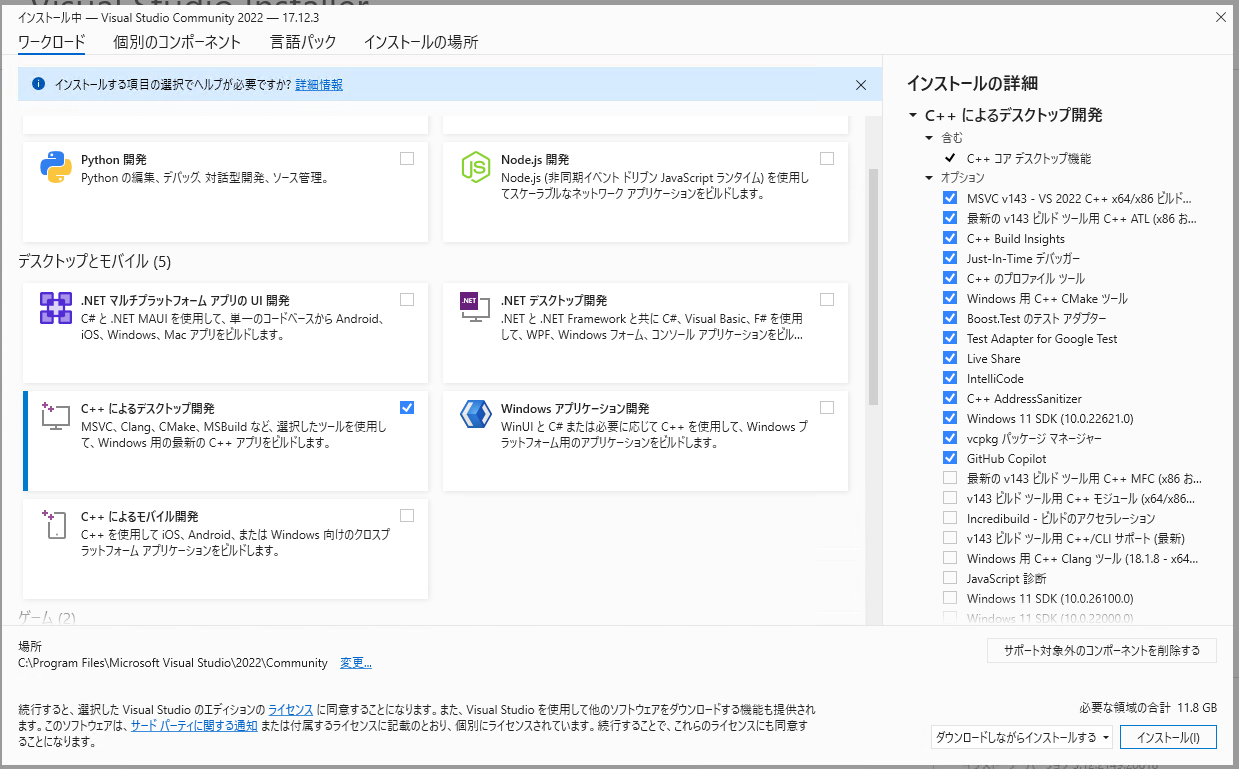
\includegraphics[width=0.8\hsize]{img/vs2022/workload.png}
    \caption{ワークロード選択画面}
\end{figure}

次に``個別のコンポーネント''より``Windows 11 SDK''の最新版を追加します。
検索欄に``Windows 11 SDK''と入力すると探しやすくて良いでしょう。
探した結果、すでに選択されている場合は、最新のものを2つ選択するようにしてください。

\begin{figure}[H]
    \centering
    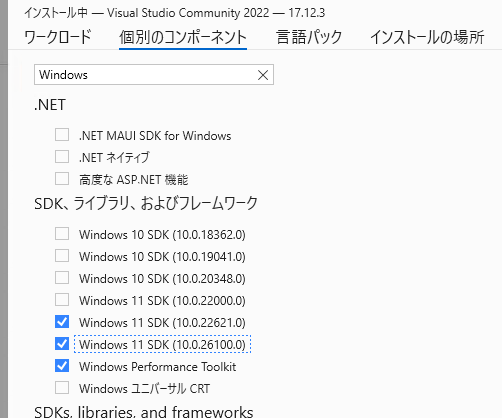
\includegraphics[width=0.7\hsize]{img/vs2022/compo_win11sdk.png}
    \caption{Windows 11 SDKの最新版の選択}
\end{figure}

次に最新のMFC用ビルドツールを追加します。
検索欄に``C++ MFC''と入力すると探しやすくて良いでしょう。
使用しているプラットフォームに合わせて（多くの場合``x86およびx64''）最新のC++ MFCビルドツールを選択してください。VisualStudio2022 であれば、 v143 になっているはずです。
Snapdragonが乗ったSurface向けにクロスコンパイルしたい場合などは、ARM64/ARM64ECなど、環境に応じたツールもインストールしてください。
基本的に``x86およびx64向け''を選択しておけば間違いないですが、まよったら画像のように全部入れてください。

\begin{figure}[H]
    \centering
    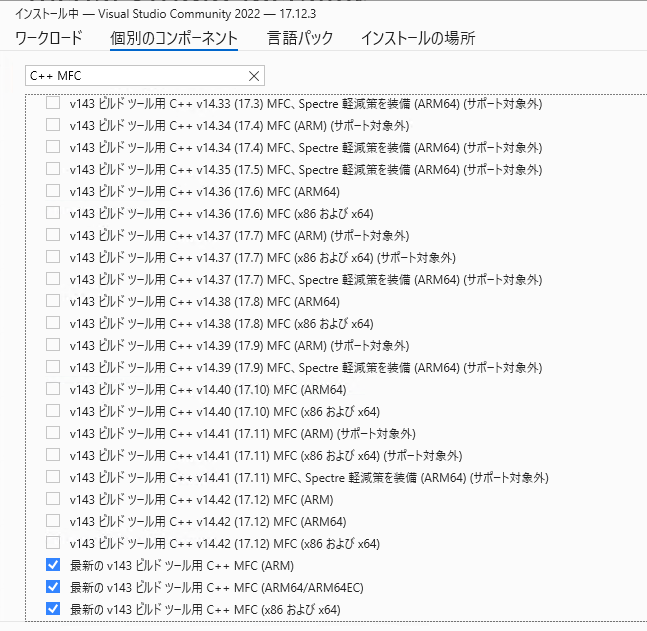
\includegraphics[width=0.8\hsize]{img/vs2022/compo_latest_mfc.png}
    \caption{プラットフォームの選択}
\end{figure}

最終的に、１～５個程度の追加パッケージが選択されているのを確認し、インストールを開始します。

\begin{figure}[H]
    \centering
    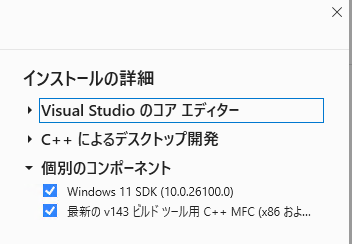
\includegraphics[width=0.6\hsize]{img/vs2022/compo_result.png}
    \caption{追加のコンポーネント一覧}
\end{figure}

\subsection{ソースコードの取得}
取得にはGitが必須です。最低限学習して、コミット、という単語の意味が分かるようにしてください。
また、submoduleも使用しているため、Gitコマンドラインでの取得を推奨します。
一発で行う場合は以下のように実行してください。

\inlinecode{git clone --recurse-submodules https://github.com/mkt-kuno/DigitShowModbus.git}

分割する場合や、更新があった場合などは

\inlinecode{git clone https://github.com/mkt-kuno/DigitShowModbus.git}

\inlinecode{git submodule update --init --recursive}

のように、分割して必要なコマンドを実行してください。詳しくはGitのドキュメントを参照してください。

\subsection{ソリューションのオープン}
VisualStudioのインストールが完了したら、ソリューションファイルを開きます。いくつか方法がありますが、最も簡単なのはVisualStudioを起動した後に``プロジェクトやソリューションを開く''を選択し、``DigitShowModbus.sln''を選択することです。

\begin{figure}[H]
    \centering
    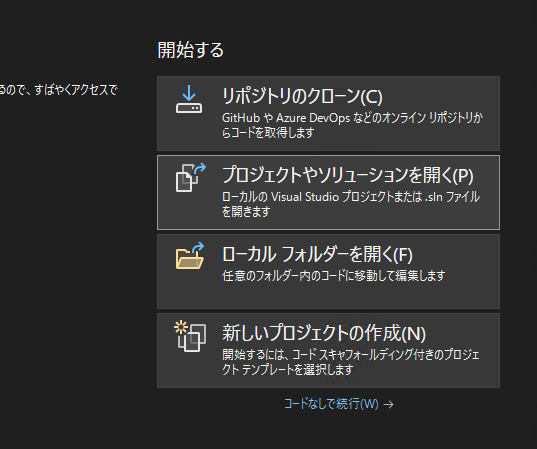
\includegraphics[width=0.6\hsize]{img/vs2022/open_solution.png}
    \caption{VisualStudio起動時初期画面}
\end{figure}

\begin{figure}[H]
    \centering
    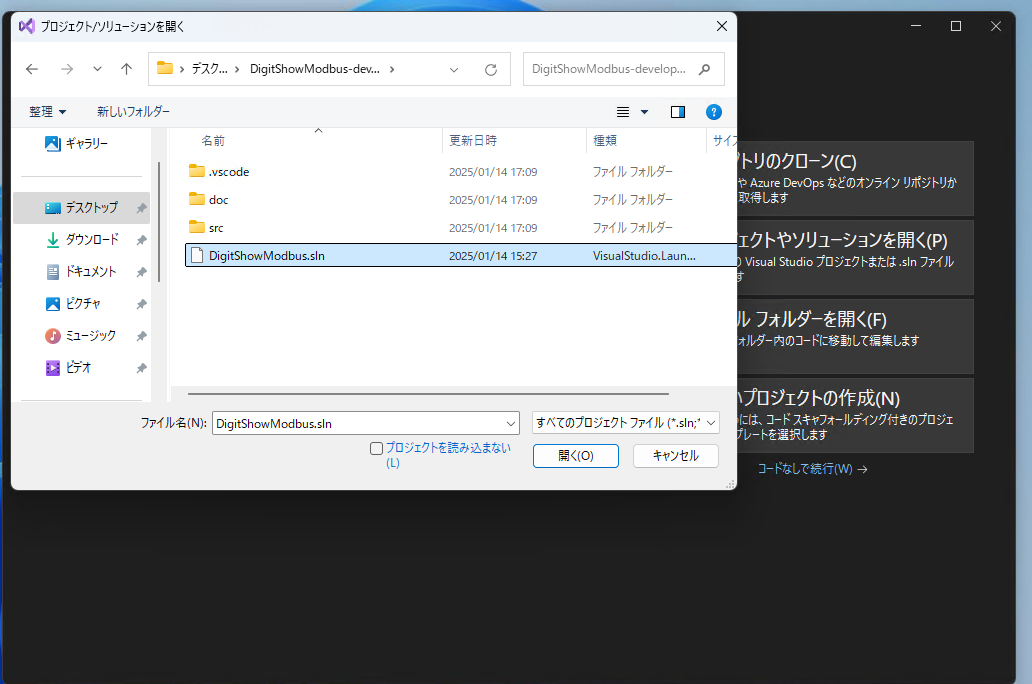
\includegraphics[width=0.8\hsize]{img/vs2022/open_sln.png}
    \caption{\inlinecode{.sln}ファイルの選択}
\end{figure}

slnファイルのダブルクリックでも開けますが、VisualStudioが複数インストールされている場合は、複雑な挙動になる可能性があります。

\begin{figure}[H]
    \centering
    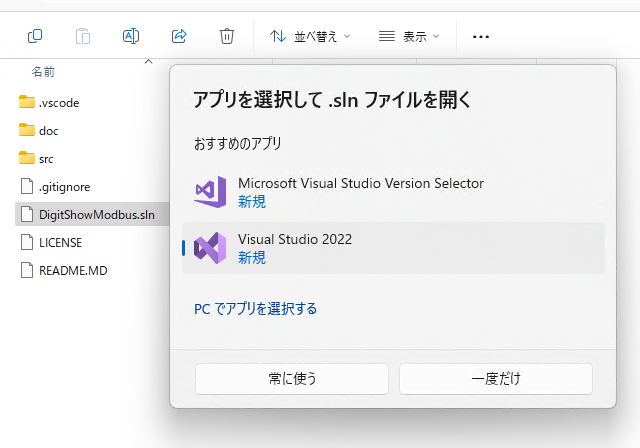
\includegraphics[width=0.8\hsize]{img/vs2022/open_sln_direct.png}
    \caption{直接選択時の挙動の一例}
\end{figure}

\subsection{ソリューションのビルド}
コードの追加時や初回運用時などは ``Debug''モードでビルドすることをお勧めします。逆にそれ以降では、ログが増えすぎることから``Release''モードでビルドすることをお勧めします。
ログの仕組みについては外部ライブラリを使用しているため``spdlog''のドキュメントを参照してください。
通常運用時は特別な理由がない限り ``x64''の``Release''を選択しておけば間違いはありません。
``spdlog''にはログレベルがあり、優先度の低いものから``trace''、``debug''、``info''、``warn''、``error''、``critical''があります。
``Release''モードでは``info''以上が出力され、``Debug''モードでは``debug''以上が出力されます。
``trace''は非常に詳細なログを出力するため、通常は使用しません。

\begin{figure}[H]
    \centering
    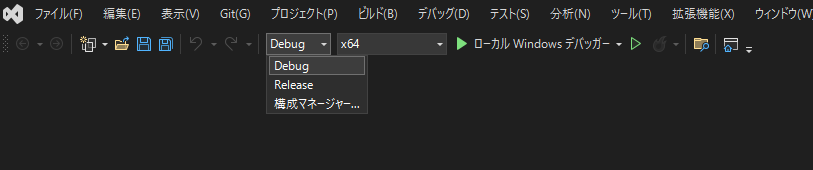
\includegraphics[width=0.8\hsize]{img/vs2022/build_mode.png}
    \caption{ビルドモードの選択}
\end{figure}

\begin{figure}[H]
    \centering
    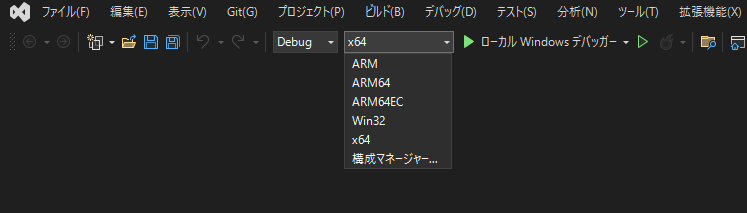
\includegraphics[width=0.8\hsize]{img/vs2022/platform_select.png}
    \caption{プラットフォームの選択}
\end{figure}

「なにもしてないのにビルドが通らなくなった」は、よくあることです。ソリューションの``リビルド''もしくは``クリーン''の後に``リビルド''してください。

\begin{figure}[H]
    \centering
    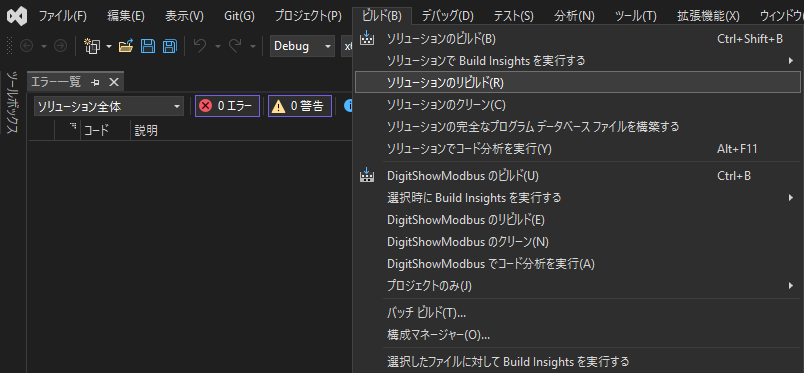
\includegraphics[width=0.8\hsize]{img/vs2022/solution_rebuild.png}
    \caption{ソリューションのリビルド}
\end{figure}

\section{コントロールの追加・修正}
\inlinecode{src/DigitShowModbusDoc.cpp} 及び \inlinecode{src/DigitShowModbusDoc.h} を起点として、\inlinecode{src/Control\_xxxx.cpp}と\inlinecode{src/Control\_xxxx.h}を編集します。
そもそもの前提知識として、自分にあった\inlinecode{C++}の教材で（なんでもいいです）、ポインタとクラスまで学んでおくことを強くお勧めします。
そこまでの知識がないと、何を書いて良いか分からなく可能性が非常に高いです。
Pythonの事前知識があればとっつきやすと思いますが、C++はPythonとは異なる部分が多いです。
正しくない記述に寄ってプログラムがクラッシュしたとしても、Pythonのようにエラー箇所がわかりやすく提示されません。

加えて、初心者レベルで良いので、Git習得を強く推奨します。Gitを使っていないと、コードのバックアップや、間違った修正を戻すことが非常に困難です。
Gitを使用していな場合、コードの変更点がわからなくなったプログラムを持って来ても、救いませんし、救えません。
上記の点に留意し、勉強したうえでコントロールを修正してください。

多くの人が修正を加えたいのは、\inlinecode{CDigitShowModbusDoc::ControlMain}での処理になると思います。
以下にIISモーターモードでの処理の例を示します。

IDが1（CONTROL\_TYPE\_PRECONSOLIDATION）の場合は、\inlinecode{Control\_PreConsolidation}を呼び出します。これは見ての通り、``Control from File''からではない先行圧密用の関数です。

IDが15（CONTROL\_TYPE\_STEP）の場合は、\inlinecode{Control\_FileCtrl\_xxxxx}関数群を呼び出します。これがメイン機能の ``Control from File''で実行されるプログラム群です。

本当に動いているか不安な場合は``Release''ビルドでもログの出る\inlinecode{spdlog::info}をどんどん追加して、ログを出力してください。

また、変なC/C++コードを追加すると、``Release''モードではコンパイラによる最適化され、コードが無視されたり、意図しない挙動になったります。
その結果``Debug''モードでは動くのに``Release''モードでは動かない、という事象が発生する可能性があります。
自分の書いたコードが不安なら``Debug''モードで動作させましょう。

\begin{tcbcodeblock}{ Control\_Motor.cpp より抜粋 }
    \begin{lstcodeblock}[language=C++]
void Control_Motor::Main()
{
	spdlog::trace("{}", __FUNCTION__);

	auto ctx = GetCDSBContext();
	if (ctx->Flag.control == FALSE)
		return;

	nlohmann::json _for_spdlog;

	spdlog::debug("MOTOR_ControlMain Ctrl Type:{}", (int)ctx->Control.type.load());

	switch (ctx->Control.type)
	{
	case CONTROL_TYPE_NONE:
		break;
	case CONTROL_TYPE_PRECONSOLIDATION:
		Control_PreConsolidation();
		break;
	case CONTROL_TYPE_STEP:
	{
		auto ctrl_step = ctx->Control.current_step.load();
		auto ctrl_step_cc = ctx->Control.Step[ctrl_step].ctrl.load();
		auto ctrl_step_args = ctx->Control.Step[ctrl_step].args;
		_for_spdlog["current_step"] = ctrl_step;
		_for_spdlog["step_num"] = ctrl_step_cc;
		for (int i = 0; i < DSM_STEPCTRL_ARGS_MAX; i++)
		{
			_for_spdlog["args"][i] = ctrl_step_args[i].load();
		}
		spdlog::info("{}:{}", __FUNCTION__, _for_spdlog.dump());

		if (ctrl_step_cc == 0)
		{
			// No Control
			Set_Speed(0.0f); // RPM->0
		}
		if (ctrl_step_cc == 1)
			Control_Motor::Control_FileCtrl_MonotonicAxialLoading();
		if (ctrl_step_cc == 2)
			Control_Motor::Control_FileCtrl_CyclicAxialLoadingStress();
		if (ctrl_step_cc == 3)
			Control_Motor::Control_FileCtrl_CyclicAxialLoadingStrain();
		if (ctrl_step_cc == 4)
			Control_Motor::Control_FileCtrl_Creep();
		if (ctrl_step_cc == 5)
			Control_Motor::Control_FileCtrl_LinearStressPathLoading();
		break;
	}
	default:
		break;
	}
}
\end{lstcodeblock}
\end{tcbcodeblock}

\section{Modbusボードについて}
\subsection{基本機能とピン配置}
ボードには3種類のコネクタがあります。HX711-ひずみ入力用コネクタ、ADS1115-電圧入力用コネクタ、GP8403-電圧出力用コネクタです。
\begin{figure}[H]
    \centering
    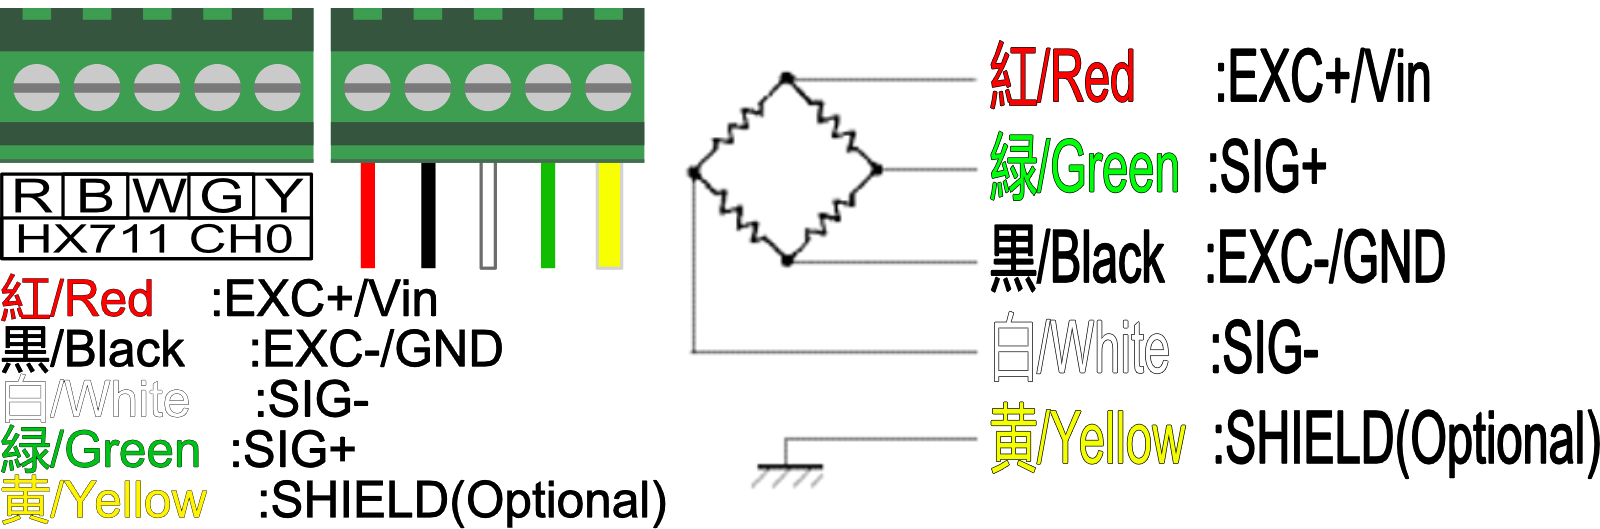
\includegraphics[width=0.8\hsize]{img/dev/modbus_hx711.png}
    \caption{HX711-ひずみ入力用コネクタの簡易説明}
\end{figure}
歪入力は4線もしくはシールド線を含む5線で接続します。Vin、GND、SIG+、SIG-、SHIELDの5本です。
シールド線は必須ではありませんが、ノイズ対策として接続することをお勧めします。
またこれらの色は一般的なロードセルの配線色に合わせていますが、必ずしも\emph{そうでない}場合があります。
\emph{必ずテスターなどで抵抗値を測定し}、正しい配線を確認してください。
一般的な抵抗値テーブルを以下に示します。
\begin{figure}[H]
    \centering
    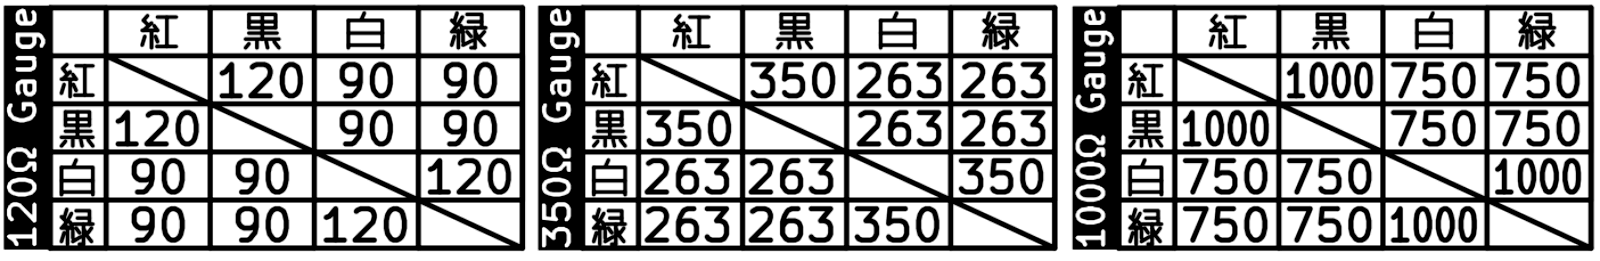
\includegraphics[width=0.8\hsize]{img/dev/gauge_table.png}
    \caption{ひずみゲージ抵抗値テーブル}
\end{figure}

ADS1115は前述の通り、電源入力のコネクタです。1ブロックにつき4入力あります。
CH10から先は16進数表記で A（10）、B（11）、C（12）、D（13）...となります。
必ず入力信号側に赤色のケーブルを接続し、ターゲットデバイスのGNDと入力チャンネル横のGNDを接続してください。逆接続するとボード、もしくはターゲットデバイスが破損します。
GP8403は電圧出力用のコネクタです。1ブロックにつき2出力あります。
必ず出力信号側に赤色のケーブルを接続し、ターゲットデバイスのGNDと出力チャンネル横のGNDを接続してください。逆接続するとボード、もしくはターゲットデバイスが破損します。
Gは予約文字でGND接続を意味します。

\begin{figure}[H]
    \centering
    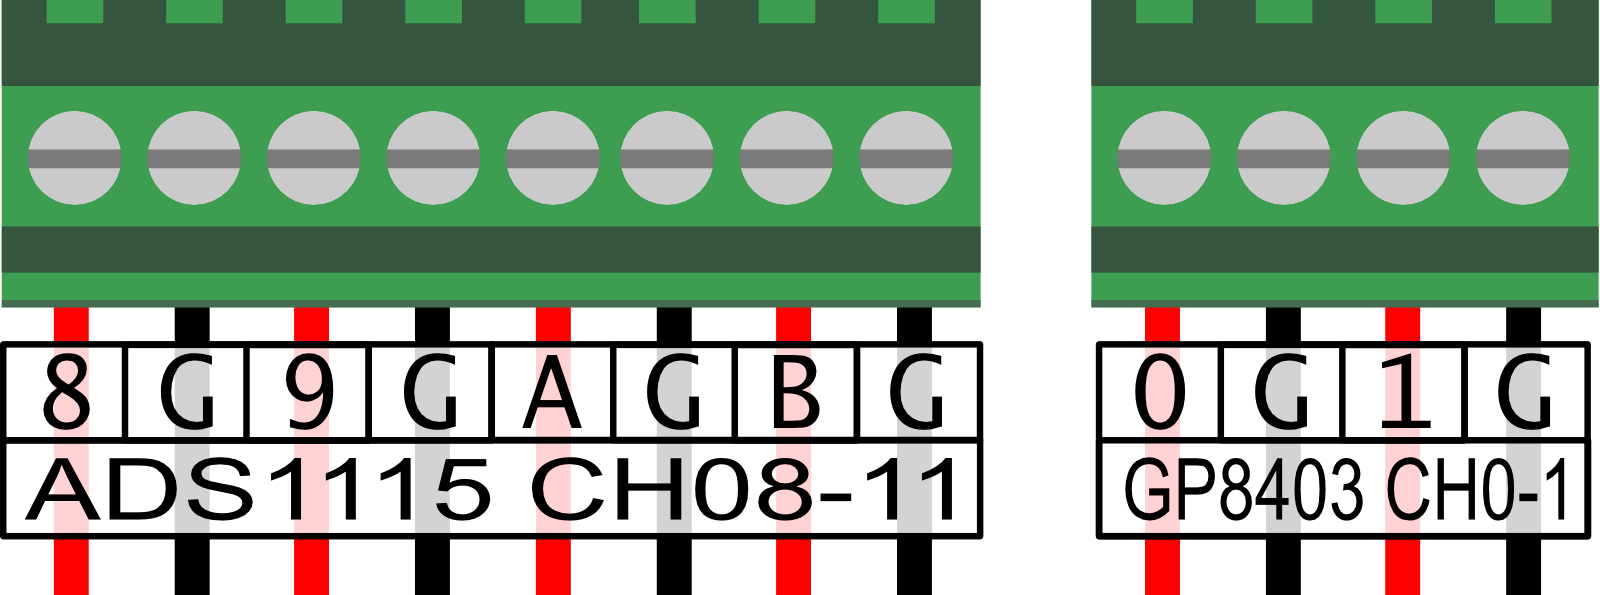
\includegraphics[width=0.8\hsize]{img/dev/modbus_other_pins.png}
    \caption{その他コネクタの簡易説明}
\end{figure}


\subsection{Modbus TCP/RTU/ASCII}
Modbusとは、1979年にModicon（現在のSchneider Electric）が開発した通信プロトコルです。
Modbusは、RS-232CやRS-485などのシリアル通信を使用するModbus RTU/ASCIIと、TCP/IPを使用するModbus TCPの2つのバージョンがあります。
TCP/IPを使用するには全台がDHCP対応でオンラインなネットワークに属しているか、静的IPで設定されたクローズドネットワークに属している必要があります。
今日日、多くの大学、会社でネットワークの管理が厳しくなっているため、本プロジェクトでは物理接続で動作が可能なModbus RTU/ASCIIを選択しました。

次にRTUとASCIIとの違いですが、どちらも同じシリアル転送、をベースとした技術です。RTUはバイナリ形式で、ASCIIはテキスト形式で通信します。
要は人間が通信内容を見たときに分かるか（テキスト形式）どうか、という感じです。
RTUはバイナリ形式で通信するため、通信速度が速く、ASCIIはテキスト形式で通信するため、通信速度が遅いです。
本プロジェクトでは将来的に通信レートが向上することに対応するため、RTUを選択しました。

\subsection{シリアル通信}
最近ではArduino、また多くの電子天秤や制御機器で``Serial''や``シリアル通信''、``UART''、``RS-232C''などの用語を見かけると思います。
厳密なことはおいておいて、これらの単語は同じ通信方式を指すと言っていいでしょう。
TX（送信）とRX（受信）これらの対によって、ホスト（Windowsなど）とデバイス（Arduinoなど）が通信を行います。
通信内容は基本的に文字列通信ですが、バイナリ通信も可能です。多くの場合文字列通信が使用されるというだけです。

ここでシリアル通信の種別について、RS-232C、RS-422、RS-485、USB-CDCなどがあります。

RS-232Cは古い規格で、シングルエンド通信のため最大通信速度が遅いですが、通信距離が長いです。
1対1の通信が可能で、通信線には最低限GND、TX+、RX+の3本が必要です。

RS-422はRS-232Cの改良版で、差動通信かつTX, RXが別れているため通信速度が速く、通信距離も長いです。
1対1の通信が可能で、通信線には最低限GND、TX+、TX$-$、RX+、RX$-$の5本が必要です。GNDを除いた4本て大丈夫な、絶縁通信もあります。

RS-485はRS-422の改良版で、差動通信でTX/RXをまとめた形のため、マルチポイント通信が可能です。
1対多の通信が可能で、通信線には最低限GND、D+、D$-$の3本が必要です。GNDを除いた2本て大丈夫な、絶縁通信もあります。

USB-CDCはシリアル通信を全部USBに乗せて通信するための規格です。USB-CDCはUSBのため、通信速度が速く、通信距離も長いです。
1対1の通信が可能で、通信線には最低限GND、D+、D$-$の4本が必要です。

例えばArduino Uno/Nanoでは、PCからArduinoボードに搭載されたFT232/CH340などのUSBシリアル変換ICまではUSB-CDCでUSB通信し、その後はFT232/CH340などのシリアル変換ICからRS-232Cでマイコンと通信を行います。
後述するYamanin（v3）ではPCからマイコンボードまで直接USBが通信線として使用されており、ロスや遅延、無駄な処理なくシリアル通信が行われます。

\subsection{シングルエンド信号と差動信号}
このような、接続できる機器の数、伝送距離、伝送速度、ノイズ耐性、電源電圧などの要素を考慮して、通信方式を選択する際に出てくるワードが、シングルエンド信号と差動信号です。
シングルエンド信号は、信号線とGNDの間で信号を送る方式です。例えばArduino等の場合、\qty{5}{\V}で動作していれば、信号線が\qty{3}{\V}以上でHIGH、\qty{1}{\V}以下でLOWというように、GNDとの電圧差で信号を判断します。
これは同時に外部から瞬間的に3V程度のノイズが乗った際に、もしくはアースやグランドが不安定になると誤動作を起こす可能性があります。
なのでテレビのリモコンなんてのは、なんとなくのGNDで動作するシングルエンド信号で動作しているため、リモコンをテレビの前に持っていかないと反応しない、方向が悪いと反応しないということがあります。
他には液晶のD-SUBなんてのは、シングルエンド信号で動作している上、あろうことかアナログ信号なので、端子の刺さりが甘かったり、端子を触ってノイズが乗ると画面が大きく乱れることがあります。

差動信号は、信号線と信号線の間の電圧差で信号を送る方式です。例えばRS-485などの場合、TX+とTX$-$の間で信号を送ります。
例えばTX+（例：\qty[print-implicit-plus]{+2}{\V}）とTX$-$（例：\qty{-2}{\V}）電圧差が4V以上ならHIGH、例えばTX+（例：-2V）とTX$-$（例：+2V）電圧差が-4V以下ならLOWというように、信号線間の電圧差で信号を判断します。
これは先ほどと違い、外部からノイズが乗っても、信号線間の電圧差が変わらない限り、誤動作を起こしにくいです。
身の回りだと、有線LANやUSB、HDMI、DVIなどが差動信号で通信しています。有線LANは 4対の通信線。USB 1.0/2.0 は 2対の通信線です。USB 3.0 は高速化の更に通信対を足しています。
要は、高速・安定の通信をするには差動信号が良い、ということです。

\subsection{フィールドネットワーク}
フィールドネットワークとは、工場や建物内の機器やセンサー、アクチュエーターなどを接続するためのネットワークです。
我々の用途も、砂・水・油・薬品を利用するため、フィールドネットワークを使用している、と言っていいでしょう。
フィールドネットワークには、Profibus、DeviceNet、EtherCAT、CC-Link、Modbus、CAN、PROFINET、EtherNet/IP、POWERLINK、Sercos、IO-Link、AS-Interface、HART、Bluetooth、Zigbee、Threadなどがあります。
あまりに多すぎますが、この殆どがライセンス絡みで有料で、ホスト側のデバイスも高価である場合が多いです。
この中で比較的安価に利用可能なのが、CAN、Modbus、Bluetoothあたりです。

CANは車載向けで多く使われてきた実績があり、車体全体のアースをGNDとすることで、1対の差動線のみで通信が可能で、一本の線が切れても通信が可能、加えて複数デバイスを接続することが可能です。
この技術は3Dプリンタにも応用され、多くのフラッグシップ3Dプリンタは、高速に動作させたいホットエンド部分につながる線を、通信速度と信頼性を保ったまま減らすため、CANを採用しています。
我々の用途の場合、CANの通信プロトコルが複雑であることと、1回あたりの通信（メッセージ）長が短い事が問題になります。

Bluetoothは無線のため、否が応でも予期しない遅延が、かつ電波環境依存で安定しない遅延時間が発生します。計測レートが\qty{1}{sample\per sec}程度ならば気になりませんが、高速計測を行う場合は、遅延が問題になるので、今回は考慮しませんでした。

残されたのがModbus、とくにRTUでした。Modbus RTUは、基本的にはRS-485を使用するため、差動信号で通信が行われ、信頼性が高いです。また、RS-485はマルチポイント通信が可能で、複数のデバイスを接続することが可能です。
しかし、RS485ではなくUSB-CDCを使用すれば、1対1通信の限定になりますが、高速通信を行うことが可能です。Arduinoなどをデバイスとするのであれば、ライブラリも多く存在し、仕様もオープンなため、開発がしやすいというメリットもあります。
またModbus TCPという上位規格があるため、物理接続がいよいよ廃れ始めた頃にTCP/IPへの以降もスムーズに進むと考えられます。
諸々の理由により、本プロジェクトではModbus RTUを採用しました。

\subsection{Modbusボード v1（Trio）/v2（Quartet）}
\begin{itemize}
    \item 開発コード：Trio（v1）/Quartet（v2）
    \item マイコン：Arduino Nano（ATmega328p）
    \item プラットフォーム：Arduino
    \item 通信方式：USBシリアル
    \item 通信プロトコル：Modbus RTU
    \item 通信速度：\qty{38400}{bps}
    \item 入力-HX711：\qty{1}{ch}/ic, 計\qty{8}{ch}, \qty{16}{\bit}精度, 128倍ゲイン,\qty{10}{\Hz}動作
    \item 入力-ADS1115：\qty{4}{ch}/ic, 計\qty{16}{ch}, \qty{16}{\bit}精度, \qty{64}{\Hz}動作（オプションで\qty{128}{\Hz}）
    \item 出力-GP8403：\qty{2}{ch}/ic, 計6/\qty{8}{ch}, \qty{12}{\bit}精度, オンデマンド動作
\end{itemize}

\subsection{Modbusボード v3（Yamanin）}
\begin{itemize}
    \item 開発コード：Yamanin（v3）
    \item マイコン：STM32F411CE（BlackPill）
    \item プラットフォーム：Zephyr RTOS
    \item 通信方式：USBシリアル
    \item 通信プロトコル：Modbus RTU
    \item 通信速度：\qty{38400}{bps}（USBダイレクトのため、何でも良い）
    \item 入力-HX711：\qty{1}{ch}/ic, 計\qty{8}{ch}, \qty{16}{\bit}精度, 128倍ゲイン, \qty{80}{\Hz}動作, 単純加算平均（8サンプル）
    \item 入力-ADS1115：\qty{4}{ch}/ic, 計\qty{16}{ch}, \qty{16}{\bit}精度, \qty{128}{\Hz}動作
    \item 出力-GP8403：\qty{2}{ch}/ic, 計\qty{8}{ch}, \qty{12}{\bit}精度, オンデマンド動作
\end{itemize}

\subsection{Modbusボード v4（Milia）}
\begin{itemize}
    \item 開発コード：Milia（v4）
    \item マイコン：Raspberry Pi Pico（RP2040）
    \item プラットフォーム：Arduino
    \item 通信方式：USBシリアル
    \item 通信プロトコル：Modbus RTU
    \item 通信速度：\qty{38400}{bps}（USBダイレクトのため、何でも良い）
    \item 入力-HX711：\qty{1}{ch}/ic, 計\qty{8}{ch}, \qty{16}{\bit}精度, 128倍ゲイン,\qty{10}{\Hz}動作
    \item 入力-ADS1115：\qty{4}{ch}/ic, 計\qty{16}{ch}, \qty{16}{\bit}精度, \qty{64}{\Hz}動作（オプションで\qty{128}{\Hz}）
    \item 出力-GP8403：\qty{2}{ch}/ic, 計6/\qty{8}{ch}, \qty{12}{\bit}精度, オンデマンド動作
\end{itemize}

\section{各ICの性能と説明}
\subsection{ひずみ入力IC：HX711}
\qty{24}{\bit}精度のADCを搭載した、内臓で128倍のゲインを持ち、\qty{10}{\Hz}もしくは\qty{80}{\Hz}のサンプリングレートを持った高精度なアナログデジタルコンバータです。
ゲージ電圧\qtyrange{1}{5}{\V}程度の、フルブリッジ式のひずみセンサーの接続に適しています。
出力される値は本来であれば、符号付き\qty{24}{\bit}精度ですが、ノイズ等により実質的な性能が\qty{16}{\bit}程度のため、本プロジェクトでは符号付き\qty{16}{\bit}精度（int16\_t/i16）として扱っています。

動作電圧が\qty{2.048}{\V}の場合の物理値と、ゲイン済み電圧、ゲイン前電圧、の関係はを表すと以下の表のようになります。

\begin{table}[htbp]
    \centering
    \caption{HX711の物理値と換算式}
    \begin{tabular}{rrrrrr}
        \toprule
        物理値 & 物理値  & 差圧（128倍）[\unit{\mV}] & 差圧[\unit{\mV}] & 電圧[\unit{\mV}] & 出力（E=2）[\unit{\mV\per\V}] \\ \midrule
        32767  & 0x7FFF &  2048 &  16 &   8 & 3.906 \\ 
        16384  & 0x4000 &  1024 &   8 &   4 & 1.953 \\
        8192   & 0x2000 &   512 &   4 &   2 & 0.977 \\
        4096   & 0x1000 &   256 &   2 &   1 & 0.488 \\
        2048   & 0x0800 &   128 &   1 & 0.5 & 0.244 \\
        0      & 0x0000 &     0 &   0 &   0 &     0 \\
        -4096  & 0xF000 &  -256 &  -2 &  -1 & -0.488 \\
        -8192  & 0xE000 &  -512 &  -4 &  -2 & -0.977 \\
        -32768 & 0x8000 & -2048 & -16 &  -8 & -3.906 \\ \bottomrule
    \end{tabular}
    \label{tab:hx711_data}
\end{table}

HX711のint16\_t（i16）物理値から\unit{\mV/\V}、もしくは\unit{\micro\upvarepsilon}への定格出力値への変換については、以下の式を使用してください。

\begin{align}
    \Delta e            &= \frac{E}{4} K\varepsilon  & \ab[\unit{\V}] \\
    \varepsilon         &= \frac{4\Delta e}{KE} & \ab[\unit{\upvarepsilon}]\\
    \frac{\Delta e}{E}  &= \frac{\mathrm{Raw}_\mathrm{i16}}{\mathrm{INT16\_MAX} \times \mathrm{HX711\_GAIN} \times \mathrm{DIFF}}  & \\
                        &= \frac{\mathrm{Raw}_\mathrm{i16}}{32767 \times 128 \times 2} & \ab[\unit{\V}]  \\
    \mu\varepsilon      &= \frac{\mathrm{Raw}_\mathrm{i16}}{\mathrm{INT16\_MAX} \times \mathrm{HX711\_GAIN} \times \mathrm{DIFF}} \times K \times 1\mathrm{E}6 & \\
                        &= \frac{\mathrm{Raw}_\mathrm{i16}}{32767 \times 128 \times 2} \times 2.0 \times 1\mathrm{E}6 & \ab[\unit{\micro\upvarepsilon}]
\end{align}
\begin{align}
    \Delta e    &: 負荷時の出力電圧 & \ab[\unit{\V}] \\
    E           &: 印加電圧 & \ab[\unit{\V}]  \\
    K           &: ゲージ率 （殆どの場合2.0） &   \\
    \varepsilon &: ひずみ & 
\end{align}

\subsection{汎用入力IC：ADS1115}
シングルエンド入力と差動入力が可能な\qty{16}{\bit}精度のADCを搭載した、I2C接続のアナログデジタルコンバータです。最大CHはシングルエンドジ4つで、差動入力で2つです。
入力電圧範囲は最大で\qtyrange[print-implicit-plus]{-6.144}{+6.144}{\V}で、計測レートは\qtyrange{8}{860}{sample\per sec}まで設定可能です。
計測レートを上げすぎると精度が下がり、計測レートを下げすぎるとチャンネル間の遅延が大きくなるため、使用される想定レートに合わせ、本プロジェクトでは\qtyrange{7}{8}{\ms\per 1ch}（\qty{32}{\ms}/\qty{4}{ch}） 程度の計測レートで使用しています。

ADS1115ののint16\_t（i16）物理値の換算表、換算式は以下の表のようになります。

\begin{table}[htbp]
    \centering
    \caption{ADS1115の物理値と換算式}
    \begin{tabular}{rrr}
        \toprule
        物理値 & 物理値  & 電圧 \\ \midrule
        32767  & 0x7FFF &  6.144 \\
        16384  & 0x4000 &  3.072 \\
        8192   & 0x2000 &  1.536 \\
        4096   & 0x1000 &  0.768 \\
        0      & 0x0000 &  0.000 \\
        -4096  & 0xF000 & -0.768 \\
        -8192  & 0xE000 & -1.536 \\
        -32768 & 0x8000 & -6.144 \\ \bottomrule
    \end{tabular}
    \label{tab:ads1115_data}
\end{table}

\begin{align}
    V   &= \frac{\mathrm{Raw}_\mathrm{i16}}{\mathrm{INT16\_MAX}} \times \mathrm{ADS1115\_RANGE} & \\
        &= \frac{\mathrm{Raw}_\mathrm{i16}}{32767} \times 6.114 & \ab[\unit{\V}]
\end{align}

\subsection{電圧出力IC： GP8403}
\qty{12}{\bit}精度のDACを搭載した、I2C接続のデジタルアナログコンバータです。最大CHは2つで、出力電圧範囲は\qtyrange{0}{10.0}{\V}です。
このICのみ入出力の指定8bitの倍数にうまく収まらないため、DFRobot社のGP8403ライブラリ互換の出力値指定方法となっています。
具体的には、指定値がuint16\_tの範囲を取り、\unit{\mV}オーダーで出力電圧を指定します。

GP8403のuint16\_t（u16）物理値の換算表、換算式は以下の表のようになります。

\begin{table}[htbp]
    \centering
    \caption{GP8403の物理値と換算式}
    \begin{tabular}{rrrr}
        \toprule
        物理値 & 物理値 & 出力電圧[\unit{\mV}] & 出力電圧[\unit{\V}] \\ \midrule
        10000 & 0x2710 &  10000 & 10.0 \\
        5000  & 0x1388 &   5000 &  5.0 \\
        2000  & 0x07D0 &   2000 &  2.0 \\
        1000  & 0x03E8 &   1000 &  1.0 \\
        100   & 0x0064 &    100 &  0.1 \\
        0     & 0x0000 &      0 &  0.0 \\ \bottomrule
    \end{tabular}
    \label{tab:gp8403_data}
\end{table}

\subsection{Arduino Nano}
Arduino Uno R3の小型版で、ATmega328P（一部、ATmega168）を搭載したマイコンボードです。シリアル変換チップを搭載しており、シリアル通信が可能です。
\qty{8}{\bit}のCPU命令、\qty{16}{\MHz}のクロック、\qty{32}{K\byte}のフラッシュメモリ（実行ファイル用ストレージ）、\qty{2}{K\byte}のRAM（メモリ）、\qty{1}{K\byte}のEEPROM（データ保存用ストレージ）を搭載しています。
Trio、Quartetの制御用マイコンとして使用されていますが、HX711を\qty{80}{\Hz}駆動で加算移動平均を適用しようとしたところ、処理が追いつかないため、Yamaninに移行する際に使用されなくなりました。
\qty{8}{\bit}マイコンはその性質上、\qty{8}{\bit}の加減算が1クロックで、\qty{16}{\bit}の加減算が2クロック、\qty{32}{\bit}の加減算が4クロックかかるため、処理が遅くなります。
特に剰余算の場合は、更に遅くなるため、単純移動平均であっても処理が間に合わなくなったものと思われます。

\subsection{WeAct Studio BlackPill STM32F411CE}
STM32F411CEを搭載したマイコンボードで、ARM Cortex-M4の\qty{32}{\bit}マイコンです。\qty{100}{MHz}のクロック、\qty{512}{K\byte}のフラッシュメモリ、\qty{128}{K\byte}のRAMを搭載しています。
先述の通り、HX711の\qty{80}{Hz}対応、加算移動平均処理に対応するためにマイコンの変更が行われました。
また、STM32F411CEは、ZephyerRTOSを使用することによってダイレクトなUSB-CDCが利用可能のため、シリアル変換チップが不要で、USBケーブルを直接接続することが可能です。
\qty{32}{bit}マイコンのため、\qtyrange{8}{32}{\bit}までの加減算が1クロックで行えるため、処理が高速になります。多くの変数が\qty{16}{\bit}以上であるため、これは強力な高速化になります。
加えて、CPUの動作周波数も6倍以上であるため、その分処理速度が向上し、パソコンからの処理を遅延なく行えることが出来るようになります。

\subsection{Raspberry Pi Pico（RP2040）}
Raspberry Pi Picoは、RP2040を搭載したマイコンボードで、ARM Cortex-M0+の\qty{32}{\bit}マイコンです。\qty{125}{MHz}のクロック、\qty{2}{M\byte}のフラッシュメモリ、\qty{264}{K\byte}のRAMを搭載しています。
RP2040は、Arduinoプラットフォームで使用することができ、Arduino Nanoと同様にUSBシリアル通信が可能です
USB CDC-ACMを使用することにより、シリアル変換チップが不要で、USBケーブルを直接接続することが可能です。
ZephyerRTOSを使用していないため、プロジェクトが簡潔にまとまっています。
コアが２つあるため、独自のルーチンやユーザーアプリケーションを並列に動作させることが可能です。
RP2040本体のADCにはエラッタがあり、\qty{8}{\bit}の精度しかないため、使用しないことをおすすめします。

\section{Webサーバー機能（開発者向け）}
\subsection{概要}
Webサーバー機能をONにすると、実行バイナリと同一ディレクトリにある ``www'' フォルダを静的コンテンツのルートディレクトリとして、Webサーバーが起動します。
多くのブラウザでは、\inlinecode{index.html} を自動的に読み込むため、\inlinecode{www/index.html} を作成しておくと、ブラウザでアクセスした際に自動的に表示されます。
これらの機能を正しく使うにはネットワークの知識が必要です。IPアドレスとはなにか、同一プライベートネットワークとはなにか、サブネットとは何かが分からない人は、まずは基礎的なネットワークの知識を学んでください。

DigitShowModbusでは、zipを利用した圧縮を透過的（自動）で行うため、よほどの理由がない限りは、開発者は圧縮済みのコンテンツ（gz、zipなど）を作成する必要はありません。
また、Modbusボードの計測データを取得したり、チャート画像を取得したり、制御コマンドを送信したりするためのWebAPIを用意しています。
これらを組み合わせると、独自のHTMLやCSS、JavaScriptを使用して、リモート監視・可視化用のWebアプリケーションを作成することができます。
これらのAPIはCORS（Cross-Origin Resource Sharing）に対応しているため、同一オリジンポリシーに縛られず、他のドメインからもアクセス可能です。

基本となるWebUIとして、\inlinecode{https://github.com/mkt-kuno/DigitShowWebview/}にて、
DigitShowModbusのWebAPIを使用したリモート監視・可視化用のWebアプリケーションのサンプルを公開しています。
Bun+React+TypeScriptで作成されており、高速に動作しますが、AIに書かせたコードも多く、安定した動作は保証できません。
複雑な表示や、高機能なダッシュボードを作成したい人は、自身でコーディングしてください。

\subsection{正常性確認API（v1）}
\inlinecode{/v1/health/} に GET リクエストを送ると、サーバーの正常性を確認できます。
状態とタイムスタンプのみがJSON形式で返されます。

\subsection{計測データの取得API（v1）}
\inlinecode{/v1/} に GET リクエストを送ると、現在の最新計測データを取得できます。
\inlinecode{localhost:80} 運用時であれば \inlinecode{http://localhost/v1/} でアクセスできます。
計測データはJSON形式で返されます。
以下は、計測データの例です。

\begin{tcbcodeblock}{計測データJSON 一部抜粋}
\begin{lstcodeblock}[]
{
  "control": {
    "cycle_state": 0,
    "mode": 0,
    "num_cyclic": 0,
    "stepctrl": {
      "args": { "00": 0.0, "01": 0.0, "02": 0.0, "03": 0.0, "04": 0.0 },
      "ctrl": 0,
      "current_step": 0
    },
    "type": 0
  },
  "current": {
    "e_p": 1.7425289154052734,
    "e_sa": 5.226467609405518,
    "e_sr": 0.0005594491958618164,
    "ea": 0.0,
    "er": 0.0050961971282958984,
    "ev": 0.010185915976762772,
    "p": 0.0,
    "q": 5.225908279418945,
    "specimen": {
      "area": 1963.29541015625,
      "diameter": 49.99745178222656,
      "height": 100.0,
      "volume": 196329.546875
    }
  },
  "flag": { "control": false, "cyclic": false, "save_data": false, "set_board": true },
  "output": { "00": { "label": "00:Motor ON/OFF", "value": 0.0 } "01": {"label": "01:Motor UP/DWN", "value": 0.0 } },
  "param": { "00": { "label": "00:q(kPa)", "value": 5.225908279418945 }, "01": { "label": "01:p'(kPa)", "value": 1.7425289154052734 } },
  "phy": { "00": { "label": "00:Load(N)", "value": 10.260002136230469}, "01": { "label": "01:ExtDisp(mm)", "value": 0.0 } },
  "raw": { "00": { "label": "00:LoadCell(i16)", "value": 42.0 }, "01": { "label": "01:LVDT(i16)", "value": -3.0 } },
  "system": { "color": "#002020" },
  "time": {
    "ctrl_delta_sec": 0.0,
    "ctrl_step_elapsed_sec": 0.0,
    "interval_ms_ctrl": 200,
    "interval_ms_disp": 100,
    "interval_ms_save": 1000,
    "save_elapsed_sec": 0.0
  }
}
\end{lstcodeblock}
\end{tcbcodeblock}

\subsection{チャート画像の取得API（v1）}
チャート画像は実機で表示されているものと同じものを取得できます。
GETリクエストのタイミングによっては、画像更新中のためにエラーが返されることがあります。
\inlinecode{/v1/img/chart\_a/} に GET リクエストを送ると、チャート画像（左）を取得できます。
\inlinecode{/v1/img/chart\_b/} に GET リクエストを送ると、チャート画像（右）を取得できます。
\inlinecode{localhost:80} 運用時であれば \inlinecode{http://localhost/v1/img/chart\_a/} でアクセスできます。

\subsection{プレビュー用データ配列の取得API（v1）}
プレビュー用データ配列は、計測データを最大点数（デフォルト：512）で保存されたものを取得できます。
必要なデータを引数としてURLエンコードしてGETリクエストを送信します。
\inlinecode{/v1/preview/} に GET リクエストを送ると、プレビュー用データ配列を取得できます。
\inlinecode{localhost:80} 運用時であれば \inlinecode{http://localhost/v1/preview/} でアクセスできます。
計測データはJSON形式で返されます。
例えば\inlinecode{time}と\inlinecode{phy\_00}を取得したい場合、
\inlinecode{http://localhost/v1/preview?time\&phy\_00} のように指定します。

以下は、プレビュー用データ配列の例です。
\begin{tcbcodeblock}{プレビュー用データ配列JSON 一部抜粋}
\begin{lstcodeblock}[]
{
    "raw_00": {
        "label": "00:LoadCell(i16)",
        "data": [
            -13.0,
            -13.0,
            -13.0,
            -13.0,
            -13.0,
            -13.0,
            -13.0,
            -13.0,
            -13.0,
            -13.0,
        ]
    },
    "time": {
        "label": "Time[s]",
        "data": [
            0.01899999938905239,
            0.04399999976158142,
            0.05999999865889549,
            0.07100000232458115,
            0.09099999815225601,
            0.10700000077486038,
            0.12300000339746475,
            0.1379999965429306,
            0.15000000596046448,
            0.1679999977350235,
        ]
    }
}
\end{lstcodeblock}
\end{tcbcodeblock}
\chapter{{\LaTeX}による本ドキュメントの編集方法}
\section{環境構築}
Dev Containerによって{\LaTeX}の開発環境をまるごとコンテナ化することで、面倒な{\LaTeX}の環境構築を回避しつつ、本ドキュメントを編集することができます。ただし、依然としてコンテナを動かすための環境構築は必須であり、ここではその方法を説明します。手順さえ踏めば、{\LaTeX}のインストールとは違って、謎のエラーに苦しむこともないはずです。

Dev Containerについてのより詳しい解説はVisual Studio Codeのウェブサイト（\url{https://code.visualstudio.com/docs/devcontainers/containers}）を参照してください。ここでの説明はこのサイトの和訳と抜粋にすぎません。

\subsection{Dockerのインストール}
\subsubsection{Windowsにインストールする場合}
Docker Desktopをインストールしてください。WindowsのエディションがHomeの場合はWSL2機能を有効にする必要があります。

\subsubsection{Windows上のWSL2（Ubuntu）にインストールする場合}
\begin{enumerate}
    \item 以下2つをインストールしてください。具体的な方法はそれぞれのウェブサイトを参照してください。
    \begin{itemize}
        \item Docker Engine: \url{https://docs.docker.com/engine/install/ubuntu/}
        \item Docker Compose: \url{https://docs.docker.com/compose/install/linux/}
    \end{itemize}
    \item \inlinecode{sudo usermod -aG docker \$USER}を実行してください。
    \item Ubuntuの再起動をかけてください。
\end{enumerate}

\subsection{Visual Studio Code（VS Code）のインストール}
\begin{enumerate}
    \item Windows上にVS Code本体をインストールしてください。
    \item VS Code上の拡張機能を以下2つインストールしてください。偽の拡張機能（マルウェアの可能性があります）に注意してください。
    \begin{itemize}
        \item Dev Conteiners extension: \url{https://marketplace.visualstudio.com/items?itemName=ms-vscode-remote.remote-containers}
        \item Remote Development extension pack: \url{https://marketplace.visualstudio.com/items?itemName=ms-vscode-remote.vscode-remote-extensionpack}
    \end{itemize}
\end{enumerate}

\subsection{Gitの設定}
WindowsもしくはWSL2（Ubuntu）上にGitがインストールされているのは前提とします。ローカルにユーザー名とメールアドレスが適切に設定されていることを確認してください。
\begin{quote}
    \inlinecode{git config --global user.name "Your Name"}

    \inlinecode{git config --global user.email "your.email@address"}
\end{quote}

Dev Containerでは、適切に設定すれば、コンテナの内部でも上手くGitを使うことができます。つまり、ここで使う仮想コンテナは\inlinecode{./doc}に構築されるコンテナですが、そのコンテナはDigitShow Modbus本体のGitまで見に行ってくれます。よって、VS Codeでドキュメントを編集しながら、そのままpush等が可能です。ここではそのための設定を行います。

詳細はVS Codeのウェブサイト（\url{https://code.visualstudio.com/remote/advancedcontainers/sharing-git-credentials}）にある通りです。「Using a credential helper」というのが楽だと思います。これはつまりGitHubのウェブサイト（\url{https://docs.github.com/ja/get-started/getting-started-with-git/caching-your-github-credentials-in-git}）を参照せよということなので、これに従ってください。

\section{作業方法}
\begin{enumerate}
    \item VS Code上でDigitShow Modbusが格納されたディレクトリを開いてください。
    \item Ctrl + Shift + Pのショートカットを利用し、「開発コンテナー：コンテナーでフォルダを開く」を選択してください。
    \item \inlinecode{./doc}ディレクトリを選択しOKを押してください。
    \item 任意の\inlinecode{.tex}ファイルを編集し、保存すると自動でコンパイルが回ります。エディタ右上の▷を押してもコンパイルが回ります。▷の右の、分割画面にルーペがついたボタンを押すと、隣にPDFを参照しながら\inlinecode{.tex}ファイルを編集できます。
\end{enumerate}

\section{{\LaTeX}を書くときのルール}
\begin{itemize}
    \item 文書の見た目（スタイル）ではなく構造（意味や役割など）を意識してください。あくまで後者が主であり、前者はそれに付随する概念です。例えば、ある部分を太字にしたいと思っても、\inlinecode{{\textbackslash}textbf}は使わないでください。太字にしたいのはそこを強調するためであり、そうであれば強調コマンド\inlinecode{{\textbackslash}emph}を使うのが理にかなったやり方です。なお、\emph{強調はゴシック体}で定義されています。変更も可能です。
    \item ダブルクオーテーションマークで括るときは、\inlinecode{"}で括るのではなく\inlinecode{``}と\inlinecode{''}で括るようにするとダブルクオーテーションマークの形が整います。出力例は次の通りです。\inlinecode{"text."}{\rightarrow}"text." \inlinecode{``text.''}{\rightarrow}``text.''
    \item 好みの問題に近いですが、和文では全角記号を使うと見た目が整うように思います。例えば括弧類（）やコロン：など。和文の中に英数字を含めなければいけない場面では臨機応変に対応しましょう。
    \item 図表や章にはラベルをつけて参照することができます。ラベルのネーミングは（技術的には）自由ですが、\inlinecode{fig:}, \inlinecode{tab:}, \inlinecode{sec:}のように、何のラベルかを冒頭で示すと便利です。参照する際には\inlinecode{{\textbackslash}cref}を使うと、例えば図を参照した際には自動的に「図 1.1」のように、表を参照した際には自動的に「表 1.1」のように出力してくれます（cleverefパッケージ）。
    \item 単位つきの数値を扱うときにはsiunitxパッケージの機能を利用すると、数値と単位との間のスペーシングなどのスタイルが整います。例えば\qty{100}{\kPa}は\inlinecode{{\textbackslash}qty\{100\}\{{\textbackslash}kPa\}}とします。あるいは\qty{1e5}{\kg.\m^{-1}.\s^{-2}}は\inlinecode{{\textbackslash}qty\{1e5\}\{{\textbackslash}kg.{\textbackslash}m{\textasciicircum}\{-1\}.{\textbackslash}s{\textasciicircum}\{-2\}\}}とします。ほかにも\qtyrange{15}{20}{\kPa}は\inlinecode{{\textbackslash}qtyrange\{15\}\{20\}\{{\textbackslash}kPa\}}と書けます。
    \item 数式を書くときは、イタリック体と立体（ローマン体）の使い分けに注意しましょう。例えばイタリック体で$ABC$と書くと$A\times B\times C$と解釈されますが、立体で$\mathrm{ABC}$と書くとABC（一つの数）と解釈されます。また、添え字も$h_\mathrm{init}$にようにして立体にすることが多々あるようです。数式モードで立体にするには\inlinecode{{\textbackslash}mathrm\{\}}を使います。
    \item TikZパッケージを使うときれいな図が描けます。使い方はオンラインマニュアル（\url{https://tikz.dev/}）を見てください。
    \item コードやファイル名、ディレクトリをインラインで書きたいときは\inlinecode{{\textbackslash}inlinecode}を定義したので、そちらを使ってください。
    \item コードブロックもかけます（listingsパッケージ）。
    \begin{tcbcodeblock}{DigitShowModbus.cpp}
        \begin{lstcodeblock}[language=C++]
// DigitShowModbus.cpp : アプリケーション用クラスの機能定義を行います。
//

#include "pch.h"
#include "framework.h"
#include "afxwinappex.h"
#include "afxdialogex.h"
#include "DigitShowModbus.h"
#include "MainFrm.h"

#include "DigitShowModbusDoc.h"
#include "DigitShowModbusView.h"

#define _USE_MATH_DEFINES
#include <math.h>
#include <fstream>
#include <filesystem>
#include <cstdlib>

#include "sqlite3.h"
#include <spdlog/sinks/rotating_file_sink.h>
#include <nlohmann/json.hpp>
#include <modbus.h>

#ifdef _DEBUG
#define new DEBUG_NEW
#endif
        \end{lstcodeblock}
    \end{tcbcodeblock}
\end{itemize}


\end{document}
